\chapter{Separation by Unknown Modulation}
\label{cha:unknown}

In the previous chapter, methods were proposed to separate highly overlapped signals, informed by an estimate of fundamental frequency \(F_0\) variation of the source to be separated.
Even though we showed that \(F_0\)  variation could be estimated from the mixture, often, it is not easy to obtain in practice.
In contrast, in this chapter, we will introduce separation methods which do not incorporate prior knowledge about the modulation. 
In fact, some of the methods operate blindly, meaning they do not require any further information about the sources except for the number of sources to be separated.
\par
In blind source separation research, many contributions were based on non-negative matrix factorization (NMF)~\cite{lee99, lee01}.
NMF quickly became one of the main scientific frameworks in the field of audio source separation with a large number of contributions.
The popularity of NMF algorithms can be explained by the intuitive way in which they work on (non-negative) time-frequency representations of the mixture signal.
Let us consider the magnitude \acs{STFT} \(\mX \in \sR_{+}^{F \times T}\) with \(F\) being the number of frequency bins and \(T\) the number of time frames.
Now, the NMF incorporates non-negative constraints to perform the separation into the sum of \(K\) latent components which are all factored into two matrices (referred to as frequency \emph{basis} \(\mW \in \sR_{+}^ { F \times K }\) and temporal \emph{activations} \(\mH \in \sR_{+}^ { T \times K }\)):

\begin{equation}
   \mathbf{X} \approx \mW \mH^{T} = \sum\limits_{k=1}^{K} \vw_{k} \circ \vh_{k}
   \label{eq:vanilla_nmf}
\end{equation}

As it can also be seen in Figure~\ref{fig:nmf}, the factorization can also be written as the sum of \(K\) outer products between two rank-one matrices \(\vw_k \in \sR^F\) and \(\vh_k \in \sR^T\).

\begin{figure}[ht]
  \centering
  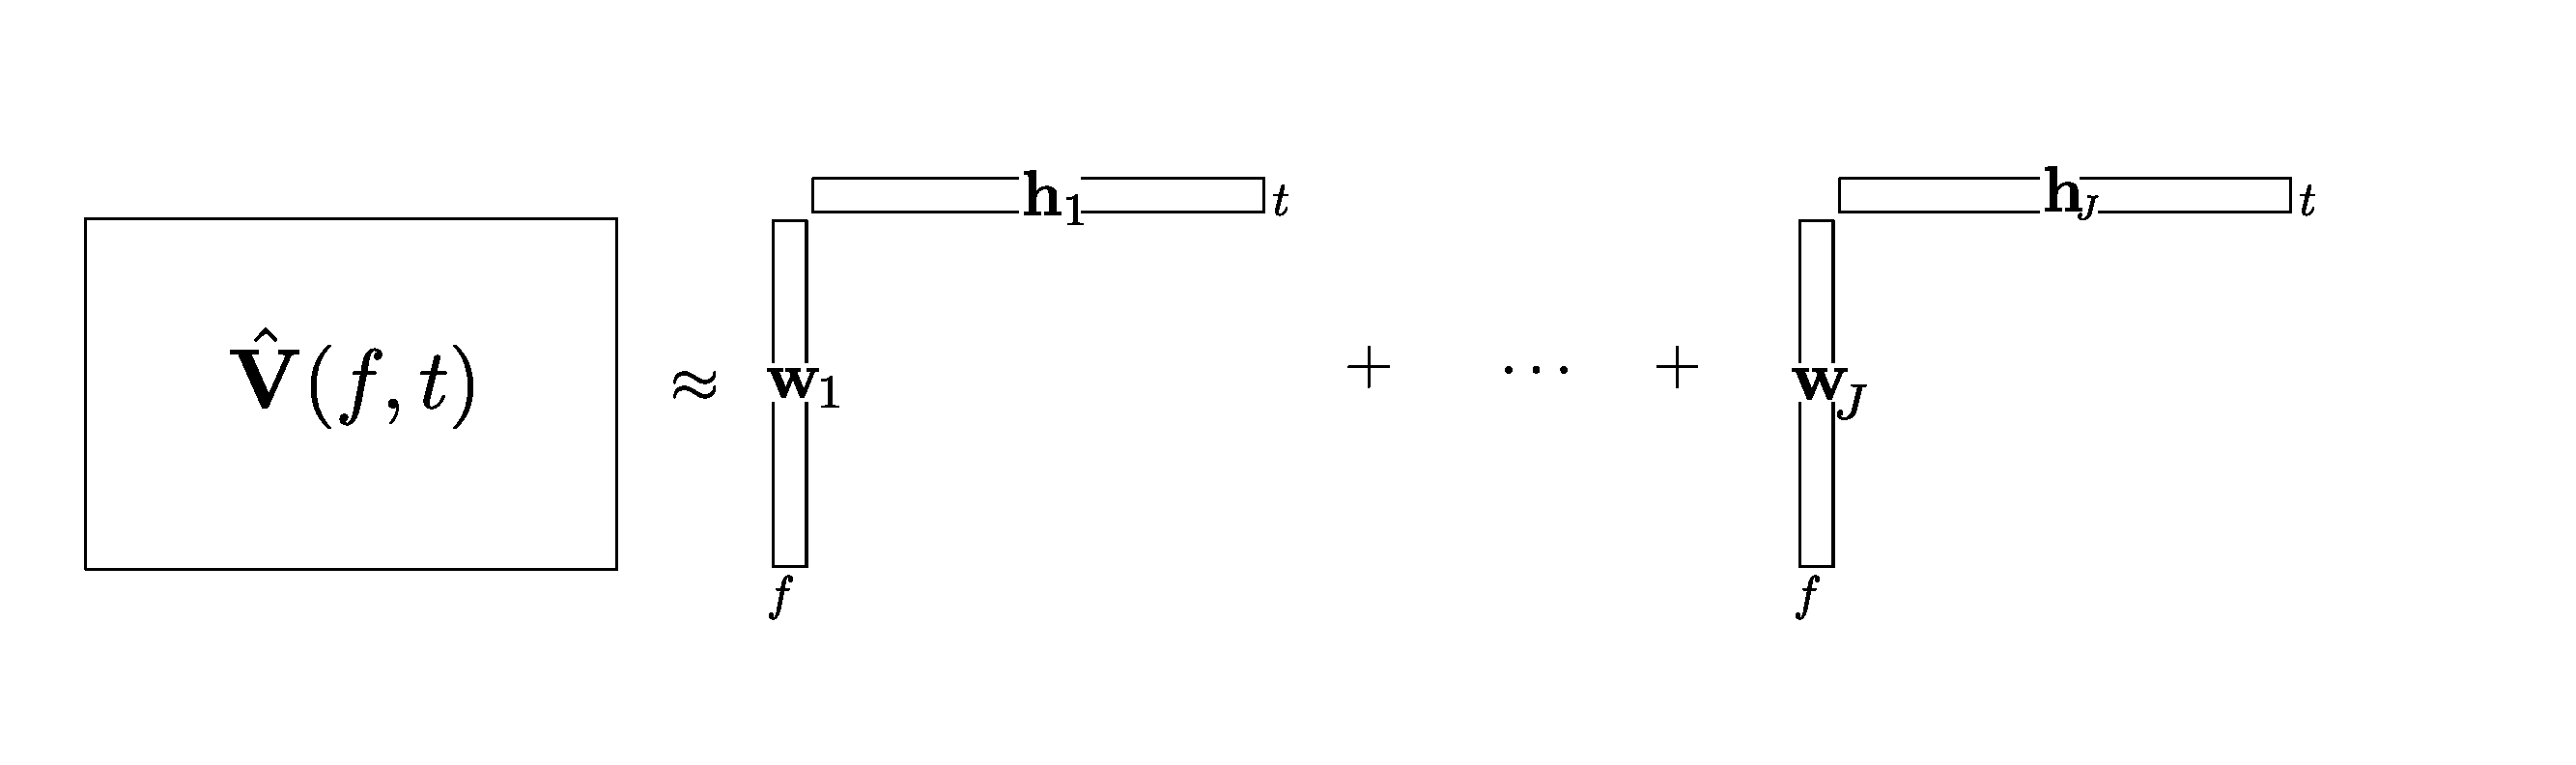
\includegraphics[width=0.9\textwidth]{Chapters/06_Separation_Unknown/figures/nmf.pdf}
  \caption{Visualization of the product of two rank-one matrices as being used in non-negative matrix factorization (NMF).}
  \label{fig:nmf}
\end{figure}

The NMF provides a rank reduction which allows decomposing mixtures into \(K\) source components.
At the same time, the factorization inherently follows specifics of music, observable in time-frequency representations: the fact that harmonic sources can be described using a pitch/tone (represented in \(\mW\)) and its duration (represented in \(\mH\)).
It is this property that also allowed to use NMF for the purpose of transcriptions~\cite{smaragdis03}.
\par
To obtain the factorization, an optimization problem needs to be solved, resulting in a non-unique solution.
Each factorization is calculated by minimizing the error between \(\mX\) and \(\mW \mH^{T}\) with respect to some cost function

\begin{equation}
  \min_{\mW,\mH^{T}} \mathrm{D}(\mX | \mW \mH) \text { subject to } \mW \geq 0 , \mathbf \mH \geq 0.
\end{equation}

In most source separation methods the beta-divergence cost function

\begin{equation}
  \mathrm{D}_{\beta} (x | y) = \frac { 1 } { \beta ( \beta - 1 ) } \left( x ^ { \beta } + ( \beta - 1 ) y ^ { \beta } - \beta x y ^ { \beta - 1 } \right) \quad \beta \in \mathbb { R } \backslash \{ 0, 1 \}
\end{equation}

is being used~\cite{fitzgerald08a}. 
For the special cases of \(\beta = 0\) and \(\beta = 1\), \(\mathrm{D}\) correspond to the Itakura-Saito (IS) and Kullback-Leibler (KL) divergence and the euclidean distance equals to \(\beta = 2\). 
To efficiently compute the optimization, an algorithm was proposed in~\cite{lee01} which makes use of simple to use multiplicative update rules, derived from the cost function. 
For further details, we refer to~\cite{cichoki09}.
\par
After factorizing \(\mX\) into \(K\) components, one can obtain \(K\) magnitude spectra.
However, \(K\) is usually selected to be larger or equal to the total number of sources.
When it is larger than the number of sources, the components can be clustered into the number of desired sources.
Often this can be achieved by some similarity metric that allows to calculate pairwise distances between the \(K\) components and the desired sources and apply \textit{k}-means clustering algorithm~\cite{spiertz09}.
A separation example is depicted in Figure~\ref{fig:nmf_separation}. 
Here the number of components \(K\) is six per source, resulting in a total number of \(K=12\). 
Each component is clustered into one of two sources to generate two estimates.

\begin{figure}[h]
  \centering
  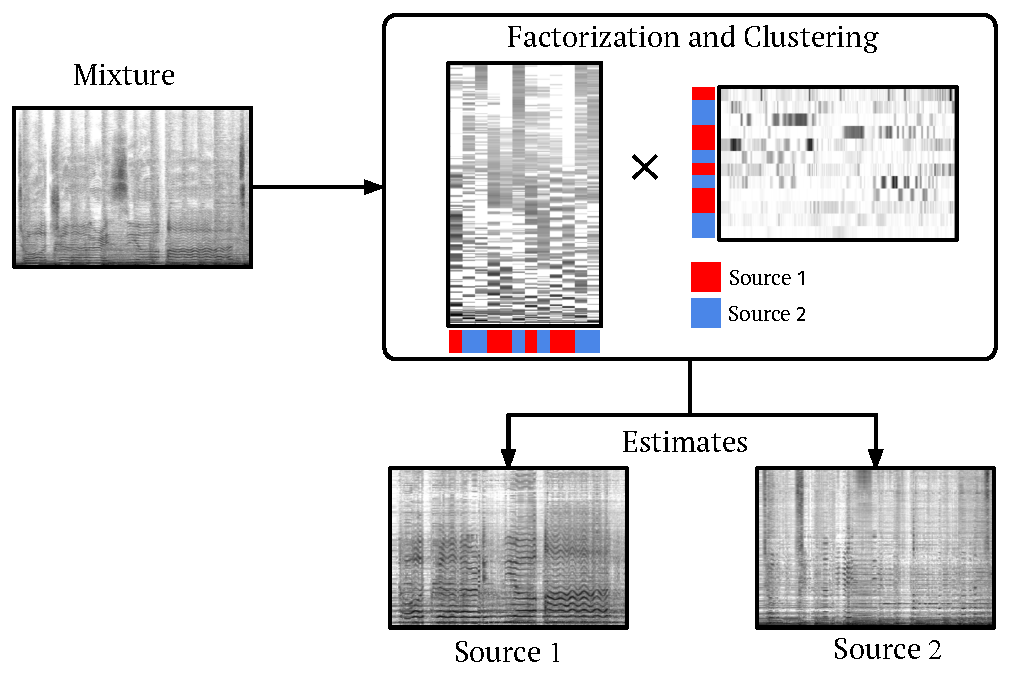
\includegraphics[width=0.8\textwidth]{Chapters/06_Separation_Unknown/figures/nmf_separation.pdf}
  \caption{Example of spectrogram based source separation using non-negative matrix factorization (NMF).}
  \label{fig:nmf_separation}
\end{figure}

It is this step that transforms the NMF into a supervised algorithm.
As for other separation methods, performed in the time-frequency domain, separation is achieved using Wiener filters or soft masks to extract the sources from the mixture~\cite{liutkus15c}.
\par
Since NMF first appeared to the source separation community in~\cite{smaragdis03} and in~\cite{vembu05}, a large variety of NMF ``flavors'' were introduced to improve certain aspects of the NMF in the application of music. 
In~\cite[Chapter 16]{vincent}, the authors describe one of the main problems of NMF which is that ``standard NMF is shown to be effective when the notes of the analyzed music signal are nearly stationary''.
As we described in Chapter~\ref{cha:highly-overlapped-signals}, this is especially problematic for pitches that incorporate vibrato.
Here, NMF-based processing suffers from its simplified model and its magnitude \acs{STFT} representation makes it harder to model these time-varying sources.
\par
To underpin this issue, we depict this problem in Figure~\ref{fig:am_tensor_nmf} which shows the factorization of a simple amplitude modulated input signal. 
The signal consists of two sinusoids which are linearly mixed. 
Both share the same carrier frequency but have different amplitude modulation rates. 
When we apply a factorization with $K=2$, one can see that NMF has difficulties to separate the two signals sufficiently and instead activates both sources in an alternating pattern.

\begin{figure}[H]
\centering
\subcaptionbox{Time Domain}%
[1\textwidth]{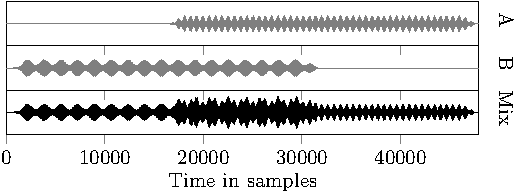
\includegraphics[width=0.84\textwidth]{Chapters/05_Separation_Known/figures/Timepdf-crop.pdf}}%
\hspace{0.2\textwidth} % separation
\subcaptionbox{Magnitude \acs{STFT}}
[1\textwidth]{% This file was created by matlab2tikz% This file was created by matlab2tikz v0.4.7 (commit 3442858e5a642c135c5e9dab6a960bee5b9c6f8d) running on MATLAB 8.2.
% Copyright (c) 2008--2014, Nico Schlmer <nico.schloemer@gmail.com>
% All rights reserved.
% Minimal pgfplots version: 1.3
%
% The latest updates can be retrieved from
%   http://www.mathworks.com/matlabcentral/fileexchange/22022-matlab2tikz
% where you can also make suggestions and rate matlab2tikz.
%
\begin{tikzpicture}[font=\small]

\begin{axis}[%
width=0.15\columnwidth,
height=3.5cm,
axis on top,
xminorgrids=true,
minor xtick={1.5,2.5},
scale only axis,
xtick={1,2},
xmin=0.5,
xmax=2.5,
ymin=0.5,
ymax=137.5,
name=plot2,
xlabel=Gain Components,
ylabel=Modulation Frequency Bins,
every axis y label/.style={at={(current axis.north east)},below=18mm,xshift=8mm},
y label style={rotate=-90},
]
\addplot [forget plot] graphics [xmin=0.5,xmax=2.5,ymin=0.5,ymax=137.5] {Chapters/05_Separation_Known/figures/AMPlots/GAS-1_scaled.png};
\end{axis}

\begin{axis}[%
width=0.15\columnwidth,
height=3.5cm,
xminorgrids=true,
minor xtick={1.5,2.5},
axis on top,
scale only axis,
xtick={1,2},
xmin=0.5,
xmax=2.5,
ymin=0.5,
ymax=145.5,
xlabel=Basis Components,
ylabel=Frequency Bins,
every axis y label/.style={at={(current axis.north east)},below=18mm,xshift=8mm},
y label style={rotate=-90},
at=(plot2.left of south west),
anchor=right of south east
]
\addplot [forget plot] graphics [xmin=0.5,xmax=2.5,ymin=0.5,ymax=145.5] {Chapters/05_Separation_Known/figures/AMPlots/GAS-2_scaled.png};
\end{axis}

\begin{axis}[%
width=0.15\columnwidth,
height=3.5cm,
xminorgrids=true,
minor xtick={1.5,2.5},
axis on top,
scale only axis,
xtick={1,2},
xmin=0.5,
xmax=2.5,
ymin=0.5,
ymax=81.5,
xlabel=Activation Components,
ylabel=Frames,
every axis y label/.style={at={(current axis.north east)},below=18mm,xshift=8mm},
y label style={rotate=-90},
at=(plot2.right of south east),
anchor=left of south west
]
\addplot [forget plot] graphics [xmin=0.5,xmax=2.5,ymin=0.5,ymax=81.5] {Chapters/05_Separation_Known/figures/AMPlots/GAS-3_scaled.png};
\end{axis}
\end{tikzpicture}%
 v0.4.7 (commit 3442858e5a642c135c5e9dab6a960bee5b9c6f8d) running on MATLAB 8.2.
% Copyright (c) 2008--2014, Nico Schlmer <nico.schloemer@gmail.com>
% All rights reserved.
% Minimal pgfplots version: 1.3
%
% The latest updates can be retrieved from
%   http://www.mathworks.com/matlabcentral/fileexchange/22022-matlab2tikz
% where you can also make suggestions and rate matlab2tikz.
%
\begin{tikzpicture}[font=\small]

\begin{axis}[%
    /pgf/number format/.cd,
           use comma,
           1000 sep={},
width=0.35\columnwidth,
height=3.5cm,
axis on top,
scale only axis,
xmin=0.5,
xmax=1497.5,
ymin=0.5,
ymax=145.5,
xlabel=Frames,
ylabel=Frequency Bins,
every axis y label/.style={at={(current axis.north east)},below=18mm,xshift=4mm},
y label style={rotate=-90},
]
\addplot [forget plot] graphics [xmin=0.5,xmax=1497.5,ymin=0.5,ymax=145.5] {Chapters/05_Separation_Known/figures/AMPlots/STFT-1_scaled.png};
\end{axis}
\end{tikzpicture}%
}%
\hspace{0.3\textwidth} % separation
\subcaptionbox{Factorization}
[1\textwidth]{% This file was created by matlab2tikz v0.4.7 (commit 3442858e5a642c135c5e9dab6a960bee5b9c6f8d) running on MATLAB 8.2.
% Copyright (c) 2008--2014, Nico Schlmer <nico.schloemer@gmail.com>
% All rights reserved.
% Minimal pgfplots version: 1.3
%
% The latest updates can be retrieved from
%   http://www.mathworks.com/matlabcentral/fileexchange/22022-matlab2tikz
% where you can also make suggestions and rate matlab2tikz.
%
\begin{tikzpicture}[font=\small]

\begin{axis}[%
/pgf/number format/.cd, use comma, 1000 sep={},
width=0.225\columnwidth,
height=3.5cm,
axis on top,
scale only axis,
xtick={1,2},
xminorgrids=true,
minor xtick={1.5},
xmin=0.5,
xmax=2.5,
ymin=0.5,
ymax=145.5,
name=plot1,
xlabel=Basis Components,
ylabel=Frequency Bins,
every axis y label/.style={at={(current axis.north east)},below=18mm,xshift=8mm},
y label style={rotate=-90},
]
\addplot [forget plot] graphics [xmin=0.5,xmax=2.5,ymin=0.5,ymax=145.5] {Chapters/05_Separation_Known/figures/AMPlots/WH-1_scaled.png};
\end{axis}

\begin{axis}[%
/pgf/number format/.cd, use comma, 1000 sep={},
width=0.225\columnwidth,
height=3.5cm,
axis on top,
scale only axis,
xminorgrids=true,
minor xtick={1.5},
xtick={1,2},
xmin=0.5,
xmax=2.5,
ymin=0.5,
ymax=1497.5,
xlabel=Activation Components,
ylabel=Frames,
every axis y label/.style={at={(current axis.north east)},below=18mm,xshift=8mm},
y label style={rotate=-90},
at=(plot1.right of south east),
anchor=left of south west
]
\addplot [forget plot] graphics [xmin=0.5,xmax=2.5,ymin=0.5,ymax=1497.5] {Chapters/05_Separation_Known/figures/AMPlots/WH-2_scaled.png};
\end{axis}
\end{tikzpicture}%
}%
\caption{Example of separating a mixture of two amplitude modulated (AM) sinusoids using non-negative matrix factorization (NMF)\\ \textbf{(a)} Mixture of two sinusoids at \SI{440}{\hertz} with AM of \SI{4.7}{\hertz} and \SI{12.6}{\hertz}, \textbf{(b)} \acs{STFT} ($FFT length = 256$), \textbf{(c)} Non-negative matrix factorization results in $\mW$ and $\mH$, after 100 iterations ($\beta = 1$).}
\label{fig:am_tensor_nmf}
\end{figure}

One way towards better separation is to increase the number of components per source, however, this introduces difficulties in the clustering.
Another method is proposed in~\cite{smaragdis04, fitzgerald05s, jaiswal13, rodriguezserrano16} which use convolutions to model shifts in components.
This leads to factorizations that are able to also model vibrato events.
However as stated in~\cite{hennequin11}, it does ``not  permit  any variation  between  different  occurrences  of  the  same event (atom), its duration and spectral content evolution being fixed''. 
Instead, they proposed a frequency-dependent activation matrices by using a source/filter-based model.
The model is based on an Auto-Regressive Moving Average (ARMA) time-varying model that allows single spectral components to be modeled along with their spectral variations. 
The model, as reported by the authors, however, does only allow for small frequency variations and fitting the ARMA model is a time-consuming process.

\section{Tensor Factorizations for Modulation Spectrograms}
\label{sub:am}

\marginpar{Parts of this subsection is also based on the work published in~\cite{stoeter14}.}

Another way to improve separation of modulated sources is the use of higher-dimensional tensor representations as a signal representation as introduced in Section~\ref{sub:modulation-analysis}.
A variety of models exist to factorize a tensor into three components and apply a similar rank reduction as in the NMF case.
Tensor factorizations are useful for applications of data with more than two dimensions.
In audio separation, tensor factorization was originally proposed to address multichannel separation as in~\cite{fitzgerald08, fevotte10, ozerov11}. 
Barker and Virtanen~\cite{barker13} were the first to propose modulation tensor representations for single-channel source separation. 
\par
As proposed by~\cite{barker13}, the non-negative tensor factorization approximates a modulation tensor \(\mV_{f, b, t}\) by a product of three matrices containing the frequency/basis \(\mW\), time/activation \(\mH\) signals, and the modulation gain for each component \(\mM\).
The product of this factorization is generally referred to as \emph{PARAFAC} product\footnote{Also known as ``Polyadic form of a tensor'', PARAFAC (parallel factors), CANDECOMP or CAND (canonical decomposition) or CP (CANDECOMP/PARAFAC)~\cite{kolda09}.}.

In the vein of the NMF factorization mentioned in Equation~\ref{eq:vanilla_nmf}, a 3-way NTF can simply be extended to:

\begin{equation}
   \mathbf{V} \approx \sum\limits_{k=1}^{K} \mathbf{w}_{k}(f) \circ \mathbf{m}_{k}(b) \circ \mathbf{h}_{k}(t).
\end{equation}

This notation is commonly used in many tensor factorization applications~\cite{kolda09}.
However, we found that it is easier to follow when the individual tensor elements are used, which is also the recommended notation proposed in~\cite{kiers00}, for  $f = 1,\ldots,F; b=1,\ldots,B;t=1,\ldots,T$:

\begin{equation}
  v_{fbt} \approx \sum_{k = 1}^{K} w_{fk} m_{bk} h_{tk}.
\end{equation}

A visualization of the three-way PARAFAC product is depicted in Figure~\ref{fig:cpd}.

\begin{figure}[!t]
  \centering
  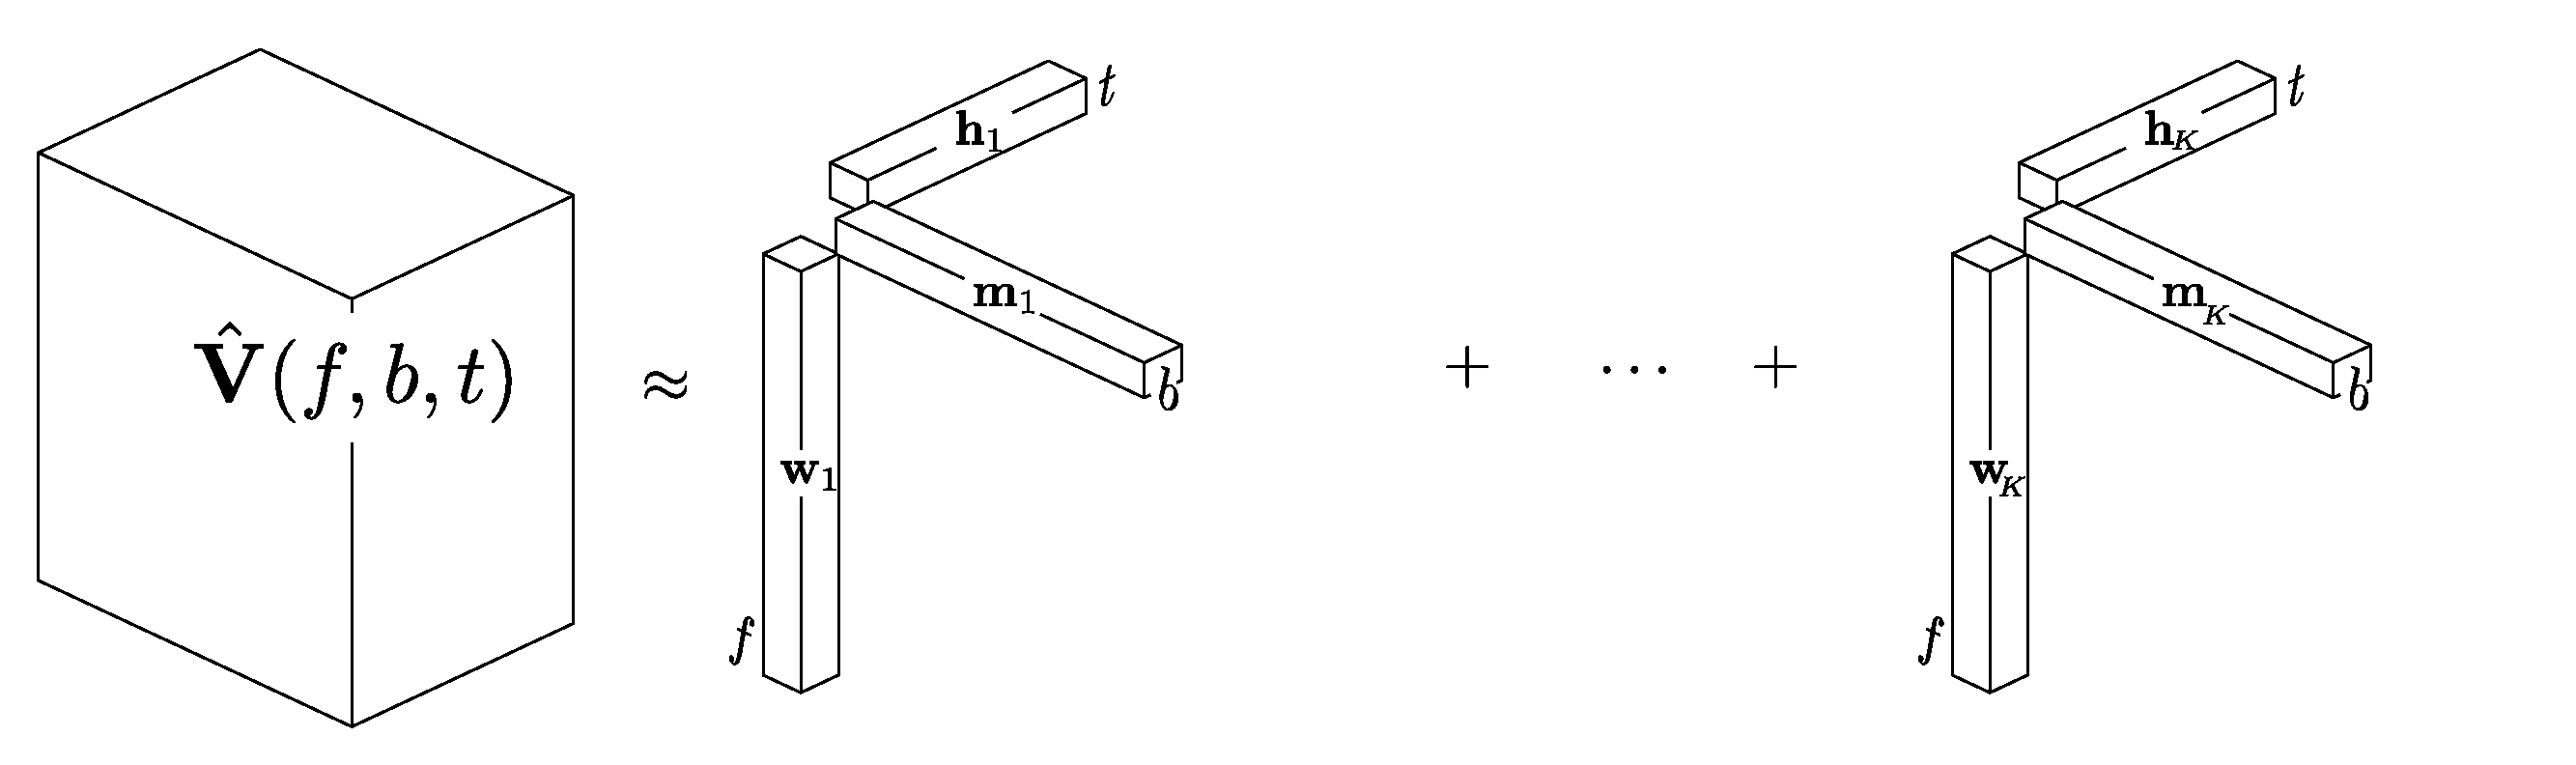
\includegraphics[width=1\textwidth]{Chapters/06_Separation_Unknown/figures/cpd.pdf}
  \caption{PARAFAC decomposition in an example for a three-dimensional tensor \(\mV\) into the sum of \(K\) outer products of three rank-one matrices.}
  \label{fig:cpd}
\end{figure}

\par
Compared to Barker and Virtanen in~\cite{barker13}, we chose to generate the modulation tensor in a way that is simpler and easier to invert. 
They used a Gammatone filter bank and rectification to model the characteristics of the human auditory system. 
We simplified the processing and used a two-stage DFT filter bank where the modulation domain is based on magnitude \acs{STFT}. 
Although this can give perceptually less optimal results, each step can be directly inverted by using the complex representation.
Barker already showed that the NTF based approach gives good results on speech signals compared to the ``standard'' NMF. 
Motivated by these results, we wondered if the modulation NTF can be used to separate two instrument mixtures by their amplitude modulation characteristics, as it is the case in the unison scenario.
\par
Thus, let us return to the example from Figure~\ref{fig:am_tensor_nmf} of two harmonic signals having the same fundamental frequency of 440~\si{\hertz}, with a stationary amplitude of 4~\si{\hertz} and 10~\si{\hertz} respectively. 
These differences now turn out to be latent in a non-negative modulation tensor representation.
In contrast to NMF, Figure~\ref{fig:am_ntf} shows valid factorizations of a unison signal using NTF.
It gives a smoother activation matrix and is able to generate the output with the separated amplitude modulations on each sinusoid. The modulation frequency gain matrix shows the two modulation frequency templates and the DC-component.

\begin{figure}[!h]
\centering
\subcaptionbox{Slice of Modulation Tensor}
[1\textwidth]{% This file was created by matlab2tikz v0.4.7 (commit 3442858e5a642c135c5e9dab6a960bee5b9c6f8d) running on MATLAB 8.2.
% Copyright (c) 2008--2014, Nico Schlmer <nico.schloemer@gmail.com>
% All rights reserved.
% Minimal pgfplots version: 1.3
%
% The latest updates can be retrieved from
%   http://www.mathworks.com/matlabcentral/fileexchange/22022-matlab2tikz
% where you can also make suggestions and rate matlab2tikz.
%
\begin{tikzpicture}[font=\small]

\begin{axis}[%
width=0.35\columnwidth,
height=3.5cm,
axis on top,
scale only axis,
xmin=0.5,
xmax=81.5,
ymin=0.5,
ymax=137.5,
xlabel=Frames,
ylabel=Modulation Frequency Bins,
every axis y label/.style={at={(current axis.north east)},below=18mm,xshift=4mm},
y label style={rotate=-90},
]
\addplot [forget plot] graphics [xmin=0.5,xmax=81.5,ymin=0.5,ymax=137.5] {Chapters/05_Separation_Known/figures/AMPlots/Tmod-1_scaled.png};
\end{axis}
\end{tikzpicture}%
}%
\hspace{0.3\textwidth} % separation
\subcaptionbox{Tensor Factorization}
[1\textwidth]{% This file was created by matlab2tikz v0.4.7 (commit 3442858e5a642c135c5e9dab6a960bee5b9c6f8d) running on MATLAB 8.2.
% Copyright (c) 2008--2014, Nico Schlmer <nico.schloemer@gmail.com>
% All rights reserved.
% Minimal pgfplots version: 1.3
%
% The latest updates can be retrieved from
%   http://www.mathworks.com/matlabcentral/fileexchange/22022-matlab2tikz
% where you can also make suggestions and rate matlab2tikz.
%
\begin{tikzpicture}[font=\small]

\begin{axis}[%
width=0.15\columnwidth,
height=3.5cm,
axis on top,
xminorgrids=true,
minor xtick={1.5,2.5},
scale only axis,
xtick={1,2},
xmin=0.5,
xmax=2.5,
ymin=0.5,
ymax=137.5,
name=plot2,
xlabel=Gain Components,
ylabel=Modulation Frequency Bins,
every axis y label/.style={at={(current axis.north east)},below=18mm,xshift=8mm},
y label style={rotate=-90},
]
\addplot [forget plot] graphics [xmin=0.5,xmax=2.5,ymin=0.5,ymax=137.5] {Chapters/05_Separation_Known/figures/AMPlots/GAS-1_scaled.png};
\end{axis}

\begin{axis}[%
width=0.15\columnwidth,
height=3.5cm,
xminorgrids=true,
minor xtick={1.5,2.5},
axis on top,
scale only axis,
xtick={1,2},
xmin=0.5,
xmax=2.5,
ymin=0.5,
ymax=145.5,
xlabel=Basis Components,
ylabel=Frequency Bins,
every axis y label/.style={at={(current axis.north east)},below=18mm,xshift=8mm},
y label style={rotate=-90},
at=(plot2.left of south west),
anchor=right of south east
]
\addplot [forget plot] graphics [xmin=0.5,xmax=2.5,ymin=0.5,ymax=145.5] {Chapters/05_Separation_Known/figures/AMPlots/GAS-2_scaled.png};
\end{axis}

\begin{axis}[%
width=0.15\columnwidth,
height=3.5cm,
xminorgrids=true,
minor xtick={1.5,2.5},
axis on top,
scale only axis,
xtick={1,2},
xmin=0.5,
xmax=2.5,
ymin=0.5,
ymax=81.5,
xlabel=Activation Components,
ylabel=Frames,
every axis y label/.style={at={(current axis.north east)},below=18mm,xshift=8mm},
y label style={rotate=-90},
at=(plot2.right of south east),
anchor=left of south west
]
\addplot [forget plot] graphics [xmin=0.5,xmax=2.5,ymin=0.5,ymax=81.5] {Chapters/05_Separation_Known/figures/AMPlots/GAS-3_scaled.png};
\end{axis}
\end{tikzpicture}%
}%
\caption{\textbf{(a)} Modulation tensor slice of a mixture of two sinusoids at \SI{440}{\hertz} with AM of \SI{4.7}{\hertz} and \SI{12.6}{\hertz} ($FFT length = 256$), \textbf{(b)}  $\mV \approx \mW \mM \mH$ Result of Non-Negative Tensor Factorization ($\beta = 1$) after 100 iterations.}
\label{fig:am_ntf}
\end{figure}
\par
A comparison of the modulation tensor approach compared to the \(F_0\) variation informed method on the unison separation scenario has been carried out in our work published in~\cite{stoeter14}.
Results indicated that the modulation tensor factorization generally performs worse than informed methods.
This is because it only considers amplitude modulations even though frequency modulations are the actual source of the modulation.
In the next section, we investigated how more complex modulation patterns can be utilized for separation.

\section{Common Fate Model for Unison Mixtures}%
\label{sec:the_common_fate_model_for_unison_mixtures}

\marginpar{This section was previously published in~\cite{stoeter16} and was revised for this thesis with permission (\textsuperscript{\textregistered}2016 IEEE).}

In this work, a novel tensor signal representation is introduced which additionally exploits similarities in the frequency direction.
We, therefore, make use of dependencies between modulations of neighboring bins.
This is similar to the proposed high-resolution non-negative Matrix Factorization model that accounts for dependencies in the time-frequency plane (HR-NMF~\cite{badeau11}).
In short, HR-NMF models each complex entry of a time-frequency transform of an audio signal as a linear combination of its neighbors, enabling the modeling of damped sinusoids, along with an independent innovation.
This model was generalized to multichannel mixtures in~\cite{badeau13a, badeau14} and was shown to provide considerably better oracle performance for source separation than alternative models in~\cite{magron15a}.
Indeed, even though some variational approximations were introduced in~\cite{badeau13} to strongly reduce their complexity, those algorithms are often demanding for practical applications.
In this work, we proposed to relax some assumptions of HR-NMF in the interest of simplifying the estimation procedure.
The core idea is to divide the complex spectrogram into modulation patches in order to group common modulation in time and frequency direction.
We call this the \emph{Common Fate Model} (CFM), borrowing from the Gestalt theory, which describes how human perception merges objects that move together over time (from~\cite{bregman90}):

\begin{quote}
``the Gestalt psychologists discovered that when different parts of the perceptual field were changing in the same way at the same time, they tended to be grouped together and seen to be changing as a group because of their common fate.'' 
\end{quote}

Bregman introduced the Common Fate theory for auditory scene analysis as the ability to group sound objects based on their common motion over time, as occurs with frequency modulations of harmonic partials.
As outlined by Bregman, the human ability to detect and group sound sources by small differences in FM and AM is outstanding.
Also, it turns out, as mentioned in Section~\ref{exploiting-slow-modulations}, that humans are especially sensitive to modulation frequencies around \SI{5}{\hertz}, which is the typical vibrato frequency that many musicians produce naturally.

\subsection{The Common Fate Transform}
\label{sub:CFT}

Let $\tilde{x}$ denote a single channel audio signal.
Its \ac{STFT} is computed by splitting it into overlapping frames and then taking the discrete Fourier transform (DFT) of each one.
Since the waveform~$\tilde{x}$ is real, the Fourier transform of each frame is Hermitian. In the following, we assume that the redundant information has been discarded to yield the \acs{STFT}.
The resulting information is gathered into an $N_{\omega}\times N_{\tau}$ matrix written~$\mX$, where~$N_{\omega}$ is the number of frequency bands and $N_{\tau}$ the total number of frames.
In this study, we will consider the properties of another object, built from $\mX$, which we call the Common Fate Transform (CFT).
\par
It is constructed as illustrated in Figure~\ref{fig:CFT}.
We split the \acs{STFT}~$\mX$ into overlapping rectangular $N_{a}\times N_{b}$ patches, regularly spaced over both time and frequency.
For reference, later in this thesis, we will call this representation the \emph{Grid STFT} (GFT).
Then, the 2D-DFT of each patch is computed\footnote{Note that since each patch is complex, its 2D-DFT is not Hermitian, thus all its entries are kept.}.
This yields an $N_{a}\times N_{b}\times N_{f}\times N_{t}$ tensor where~$N_{f}$ and~$N_{t}$ are the vertical and horizontal positions for the patches, respectively.
\par
As can be seen, the CFT is basically a further short-term 2D-DFT taken over the ``standard'' \acs{STFT}~$\mX$.
One of the main differences compared to modulation spectrograms is that the CFT is computed using the complex \acs{STFT}~$\mX$, and not a magnitude representation such as $\left|\mX\right|$.
As we will show, this simple difference has many interesting consequences, notably that the CFT is invertible: the original waveform~$\tilde{x}$ can be exactly recovered by cascading two classical overlap-add procedures.
Another difference is that the patches span several frequency bins, \emph{i.e.} we may have~$N_{a}>1$.
This contrasts with the conventional modulation spectrogram, that is defined using one frequency band only.

\begin{figure}[t]
\centering
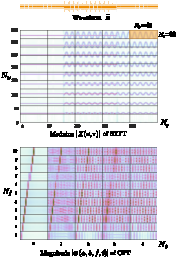
\includegraphics[width=0.8\textwidth]{Chapters/06_Separation_Unknown/figures/CFT}
\caption{Common Fate Transform. For convenience, the splitting of the STFT
into patches has been depicted without overlap, but overlapping patches are used in practice\label{fig:CFT}. \textsuperscript{\textregistered}2016 IEEE.}
\end{figure}

\subsubsection{A Probabilistic Model for the CFT}

\label{ssub:separation}

When processing an audio signal~$\tilde{x}$ for source separation, it is very common to assume that all time-frequency (TF) bins of its \acs{STFT} are independent~\cite{fevotte09, duong10, ozerov12, liutkus11t}.
This is often the consequence of two different assumptions.
The first one is to consider that all frames are independent, thus leading to the independence of all entries of the \acs{STFT} that do not belong to the same column. The second one is related to the notion of stationarity:
roughly speaking, the Fourier transform is known to decompose stationary signals into independent components.
As a consequence, when the signals are assumed to be \emph{locally stationary}, it is theoretically sound to assume that all the entries of
their \acs{STFT} are independent.

Still, both assumptions can only be considered as approximations.
First, adjacent frames are obviously not independent, notably because of the overlap between them. 
Second, the stationarity assumption is only approximate in practice, especially when percussive elements are found in the audio, leading to strong dependencies among the different frequency bins. 
Let $\{ \mX_{ft}\} _{f,t}$ denote all the $N_{a}\times N_{b}$ patches taken on the \acs{STFT} to compute the CFT, as depicted in Figure~\ref{fig:CFT}. 
The probabilistic model we choose is the combination of \emph{three} different assumptions made on the distribution of these patches\footnote{A forth assumption made in~\cite{stoeter16} refers to the joint distribution of all entries of each patch which are $\alpha$-stable~\cite{samoradnitsky94}.}.

\begin{enumerate}[leftmargin=0cm,itemindent=.5cm,labelwidth=\itemindent,labelsep=0cm,align=left]
\item All patches are independent. 
Just as the classical locally stationary model~\cite{liutkus11t} assumes independence of overlapping frames, we assume here independence of overlapping patches. 
Due to the overlap between them, this assumption is an approximation, and one may wonder what the advantage is of dropping independent frames for independent patches. 
The answer lies in the fact that the latter permits us to model phase dependencies between neighboring \acs{STFT} entries, and also to model much longer-term dependencies, as required for instance by deterministic damped or frequency-modulated sinusoidal signals.\label{enu:assumption_independent_patches}
\item Each patch is \emph{stationary}: its distribution is assumed invariant under translations in the TF plane. 
This is where we do not assume independence, but on the contrary, expect dependencies among neighboring \acs{STFT} entries. 
Our approach assumes this happens in a way that only depends on the relative positions in the TF plane. It can easily be shown that mixtures of damped sinusoids have this property.
Assuming stationarity not only over time but over both time and frequency also permits us to naturally account for mixtures of frequency-modulated sounds. 
In short, we assume that throughout each patch, we observe one coherent \acs{STFT} ``texture''. 
The difference with the HR-NMF model is that we have independent and identically distributed (i.i.d.) innovations for one given patch, whereas HR-NMF model has more variability. 
However, taking overlapping patches somehow compensates for this limitation.\label{enu:assumption_stationary}
\item All entries of the Fourier transform of each patch are assumed to be asymptotically independent, as the size of the patch gets larger.
This rather technical condition, often tacitly made in signal processing studies, permits efficient processing in the frequency domain.\label{enu:assumption_harmonisable}
\end{enumerate}

Under those assumptions, all entries of the CFT are independent (assumptions~\ref{enu:assumption_independent_patches} and~\ref{enu:assumption_stationary})\footnote{This result is the direct generalization of~\cite[th. 6.5.1]{samoradnitsky94} to multi-dimensional stationary processes.} where $P\left(a,b,f,t\right)$ is a non-negative Tensor with dimensions $N_{a}\times N_{b}\times N_{f}\times N_{t}$ that we call the \emph{modulation density}. 
In the general case, it can basically be understood as the energy found at $\left(a,b\right)$ for patch $\left(f,t\right)$, just like more classical power spectral densities describe the spectro-temporal energy content of the \acs{STFT} of a locally stationary signal.

\subsubsection{Interpretation of the CFT as Filterbank}
\label{sub:interpretation}

An alternative interpretation of the CFT can be obtained by regarding the 2D-DFT as two subsequent 1D-DFTs. 
If the transform in frequency direction (DFT-F) is applied first, it is equivalent to a partial inverse DFT plus time reversal. 
If the time reversal would be undone and an overlap-add would be applied, the output would correspond to a subband representation with a frequency resolution of $N_\omega / N_a$. 
Each of the $N_a$ final transformations (DFT-T) in one patch takes output values from $N_b$ DFT-Ts with equal indices. 
This corresponds to a splitting into poly-phase components with downsampling factor $N_a$ of the time signal obtained by placing the output frames from the DFT-Ts in a row.
Thus, the outputs of the DFT-Fs have a very high frequency resolution of $N_\omega N_b$ but contain aliasing components from the downsampling.
\par
This interpretation of the CFT gives some indications for its benefits in the separation of modulated sources. 
Due to the poly-phase representation, it has a relatively high temporal resolution. 
The periodicities in the spectra caused by downsampling make the CFT relatively independent of frequency shifts, so that, for example, the output patch of a single sinusoidal sweep is mainly influenced by the sweep rate.

\subsection{Signal Separation}
Now, let us assume that the observed waveform is actually the sum of~$K$ underlying components~$\{ \tilde{s}_{k}\} _{k=1,\dots,K}$.
Due to the linearity of the CFT, this can be expressed in the CFT domain as:
$$
\forall\left(a,b,f,t\right),x\left(a,b,f,t\right)=\sum\nolimits_{k}s_{k}\left(a,b,f,t\right).
$$
If we adopt the model presented above for each source and use the stability property, we have:
$$
\mV\left(a,b,f,t\right)\sim \sum\nolimits_{k}P_{k}\left(a,b,f,t\right),
$$
where $P_{k}$ is the modulation density for component~$k$.
The resulting waveforms are readily obtained by inverting the CFT.\@
As can be seen, we now need to estimate the modulation densities~$\{ P_{k}\}_{k}$ based on the observation of the mixture CFT~$x$, similarly to the estimation of the sources' Power Spectral Densities (PSD)
in source separation studies.

\subsubsection{Factorization Model and Parameter Estimation}
\label{sub:NTF}

In order to estimate the sources' modulation densities, we first impose a factorization model over them, so as to reduce the number of parameters to be estimated. 
In this study, we set:

\begin{equation}
\mP_{abft} \approx \sum_{k=1}^{K}a_{abfk}h_{tk},\label{eq:NTF_model}
\end{equation}
for $a=1,\ldots,N_a;b=1,\ldots,N_b;f=1,\ldots,N_f;t=1,\ldots,N_t;k=1,\ldots,K$ non-negative tensors, respectively. 
We call this a \emph{Common Fate Model}. 
Intuitively, $\mA \triangleq \{a_{abfk}\}_{a,b,f,k}$ is a modulation density template that is different for each frequency band~$f$, and that captures the long term modulation profile of each source around that frequency.
Then, $\vh \triangleq \{h_{tk}\}_{t,k}$ is an activation vector that indicates the strength of source on the patches located at temporal position~$t$.
The factorization model is depicted in Figure~\ref{fig:cfm}.
We also experimented with other two and three-factor combinations but never got any promising results, suggesting that our proposed NMF-like model is a good choice.

\begin{figure}[!htbp]
\centering
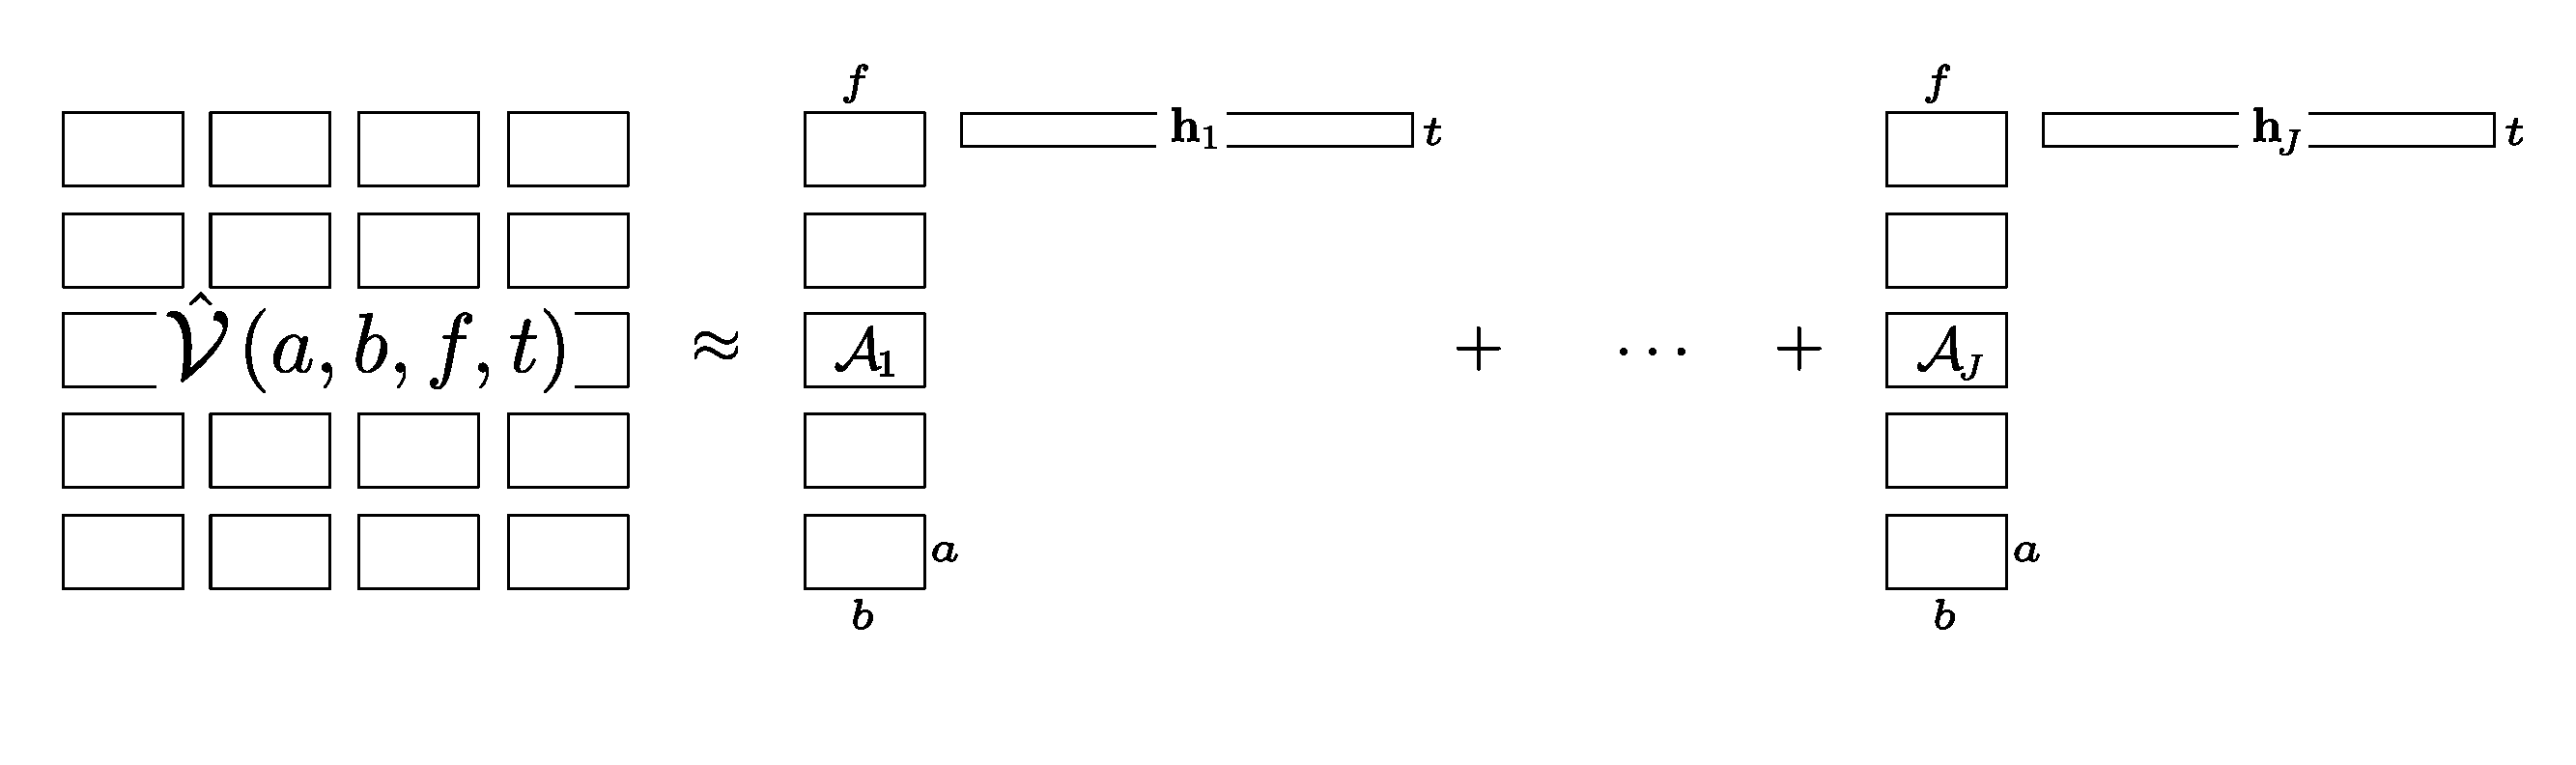
\includegraphics[width=0.9\columnwidth]{Chapters/06_Separation_Unknown/figures/cfm.pdf}
\caption{Visualization of the Common Fate factorization model (CFM).}
\label{fig:cfm}
\end{figure}

Learning those parameters can be achieved using the non-negative tensor factorization (see e.g.~\cite{cichoki09,ozerov12,smaragdis14} for an overview), except that it is applied to the CFT instead of the \acs{STFT}, and that the particular factorization to be used is~\eqref{eq:NTF_model}.

In essence, it amounts to estimating the parameters~$\{ A_{k},H_{k}\}$ so that the modulus of the CFT is as close as possible to~$\sum_{k}P_{k}$, with some particular cost function as a data-fit criterion called a $\beta$-divergence and which includes Euclidean, Kullback-Leibler and Itakura-Saito as special cases~\cite{fitzgerald08a}. 
As usual in non-negative models, each parameter is updated in turn, while the others are kept fixed.
We provide the multiplicative updates in Algorithm~\ref{alg:Fitting-NTF}.
After a few iterations, the parameters can be used to separate the sources using the Wiener filter as described in~\cite{liutkus15}.

\begin{algorithm}
With $v=\left|x\right| \forall a,b,f,t v(a,b,f,t) = |x(a,b,f,t)|$ and always using the latest
parameters available for computing
 $\hat{P}\left(a,b,f,t\right)=\sum\limits_{k=1}^{K}A_{k}\left(a,b,f\right)H_{k}\left(t\right)$,
iterate:
\[
A_{k}\left(a,b,f\right)\leftarrow A_{k}\left(a,b,f\right)\tfrac{\sum_{t}v\left(a,b,f,t\right)\hat{P}\left(a,b,f,t\right)^{\cdot\left(\beta-2\right)}H_{k}\left(t\right)}{\sum_{t}\hat{P}\left(a,b,f,t\right)^{\cdot\left(\beta-1\right)}H_{k}\left(t\right)}
\]
\[
H_{k}\left(t\right)\leftarrow H_{k}\left(t\right)\tfrac{\sum_{a,b,f}v\left(a,b,f,t\right)\hat{P}\left(a,b,f,t\right)^{\cdot\left(\beta-2\right)}A_{k}\left(a,b,f\right)}{\sum_{a,b,f}\hat{P}\left(a,b,f,t\right)^{\cdot\left(\beta-1\right)}A_{k}\left(a,b,f\right)}.
\]
\caption{Fitting parameters of the non-negative CFM~\eqref{eq:NTF_model}.\label{alg:Fitting-NTF}}
\end{algorithm}

\subsection{Experiments}
\label{sec:experiment}

In this section, we present separation experiments utilizing CFM and compare it with other methods.

\begin{table*}[ht!]
  \centering
  \scriptsize
\begin{tabular}{ llll }
    \toprule
    Method & Signal Representation & Factorization Model \\
    \midrule
    CFM~\cite{stoter16} & \acs{STFT} $\rightarrow$ Grid Slicing $\rightarrow$ 2D-DFT & $V(a,b,f,t) = P(a,b,f)\times H(t)$ \\
    NMF~\cite{virtanen07} & \acs{STFT} & $V(f,t) = W(f)\times H(t)$ \\
    HR-NMF~\cite{badeau13} & Output of any filterbank (\acs{STFT}, MDCT, \ldots)  & AR filtering of NMF excitation \\
    MOD~\cite{barker13} & \acs{STFT} $\rightarrow$ $|\ldots|$ $\rightarrow$ \acs{STFT} along each bin & $V(f,m,t) = W(f)\times A(m)\times H(t)$ \\
    CFMM & \acs{STFT} $\rightarrow$ $|\ldots|$ $\rightarrow$ Grid Slicing $\rightarrow$ 2D-DFT & $V(a,b,f,t) = P(a,b,f)\cdot H(t)$ \\
    CFMMOD & \acs{STFT} $\rightarrow$ $|\ldots|$ $\rightarrow$ Grid Slicing $\rightarrow$ 2D-DFT & $V(a,b,f,t) = P(a,b,f)\cdot H(t)$ \\
    \bottomrule
\end{tabular}
\caption{Overview of the evaluated algorithms.}
\label{tab:methods}
\end{table*}

\subsubsection{Synthetic Example}
\label{sub:Synthentic_Examples}

To illustrate the CFT representation, we processed a mixture consisting of two sinusoidal sources. 
One source is a pure sine wave of fundamental frequency \SI{440}{\hertz} whereas the other is frequency modulated by a sinusoid of \SI{6.3}{\hertz}. 
In the first step, a \acs{STFT} with a DFT-length of 1024 samples and a hop-size of 256 samples was processed at a sample rate of 22.05~kHz. 
Patches of size $(N_a, N_b) = (32, 48)$ (not respecting overlaps) were then taken from the \acs{STFT} output. 
Figure~\ref{fig:CFT} in Section~\ref{sub:CFT} then shows the Common Fate Transform for the mixture. 
One can see that the CFT representation shows distinct patterns across time, suggesting that the factorization is able to separate the sources. 
Furthermore, if we now look at a smaller excerpt of the same synthetic example, depicted in Figure~\ref{fig:gridplot}, we can also observe the additivity property of the common fate representations.

\begin{figure}[!h]
\centering
    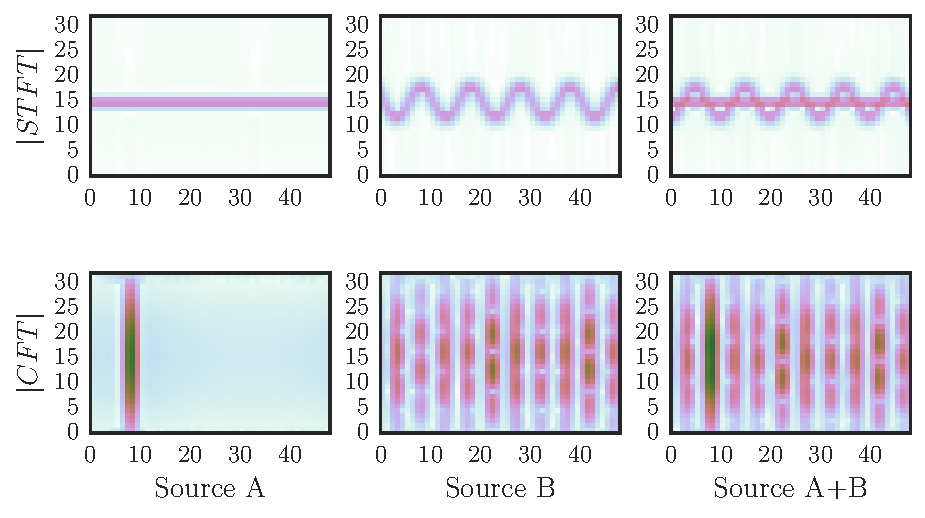
\includegraphics[width=0.9\textwidth]{Chapters/06_Separation_Unknown/figures/gridplot.pdf}
\caption{Examples of patches of size $(N_a, N_b) = (32, 48)$. The upper row shows the \acs{STFT} output, the lower row the corresponding Common Fate Transform (CFT).}
\label{fig:gridplot}
\end{figure}

\subsubsection{Objective Evaluation on Unison Instrument Mixtures}

To evaluate the proposed method, five musical instrument samples were selected from the Unison Separation Dataset~\cite{oss_unison} --- all of them feature vibrato: 
violin, cello, tenor sax, English horn, and flute. 
It is important to note that vibrato techniques differ between these instruments: 
whereas the English horn and the flute only produce a very subtle modulation, the violin and tenor sax have powerful frequency modulations with a higher modulation frequency as well as a higher modulation index. 
All samples last about three seconds. 
We then generated a combination of ten mixtures of two instruments, each one generated with a simple SourceA --- SourceB --- (SourceA + SourceB) scheme. Data were encoded in 44.1 kHz / 16 bit.
We compared the separation performance of six different methods, summarized in Table~\ref{tab:methods}:
\begin{description}[style=unboxed,leftmargin=0cm]
\item[CFM] For the CFM model, we took an \acs{STFT} with frames of 1024 samples and a hop-size of 512 samples. The resulting complex \acs{STFT} was then split into a grid of patches of size $(N_a, N_b) = (4, 64)$, each having a half-window overlap in both dimensions.
\item[MOD] We implemented a modified version of~\cite{barker13} where for the sake of comparability, we used a \acs{STFT} instead of a gammatone filterbank. A DFT length of 1024 and a hop-size of 512 samples were chosen. After taking the magnitude value, a second \acs{STFT} of size 32 and hop-size 16 samples was computed for each frequency.
\item[CFMMOD] We selected patch sizes of $(N_a, N_b) = (1, 64)$ and modified the representation so that the magnitude was applied before computing the 2D-DFT.\@ This permits to compare the advantage of our proposed factorization model~(\ref{eq:NTF_model}) over MOD, when using the same kind of energy-modulation representation in both cases.
\item[CFMM] For comparing the influence of computing modulations over complex \acs{STFT} or magnitude \acs{STFT}, we tried our factorization model when the magnitude of the \acs{STFT} is taken before 2D-DFT, with patches of the same size as for the CFM method.
\item[NMF] We took a ``standard'' NMF based method~\cite{virtanen07}. We highlight that taking a \acs{STFT} with frames of length 1024 would not make a fair comparison, because the CFM model actually results in a larger frequency resolution. Therefore a comparable NMF is based on an \acs{STFT} of DFT-length 32768.
\item[HR-NMF] See description in~\cite{magron15a}.
\end{description}
All factorizations ran for 100 iterations and were repeated five times. We chose $k=(2,\ldots,6)$ components for each factorization. For $k > 2$ we used oracle clustering to show the upper limit of SDR which can be achieved.

We ran the performance evaluation by using BSSeval~\cite{vincent06}. 
The results of Signal to Distortion Ratio (SDR), Signal to Interference Ratio (SIR), and Signal to Artifacts Ration (SAR) are depicted in Figure~\ref{fig:boxplot_overall}. 
Results indicate that the CFM model performs well in all measures. 
However, in terms of SIR, the results of HR-NMF are better than CFM method. 
The results for CFMMOD and CFMM indicate the positive influence of the CFM factorization compared to~\cite{barker13}.
The results of CFMM indicate that the complex CFT lead to better results. 
NMF did perform surprisingly well, which may only hold for our test set, where each source is active for a long period. 
This results in a cyclic stationary vibrato, revealing spectral side lobes at such a high resolution. 
With more than one component per source, the results of CFM do improve, but it can be seen that more than two components ($k=4$) will not increase the SDR values as indicated in Figure~\ref{fig:iterations}. 
The separation results and a full Python implementation of the CFM algorithm can be found on the companion website~\footnote{\url{github.com/aliutkus/commonfate}}.

\begin{figure}[ht!]
\centering
        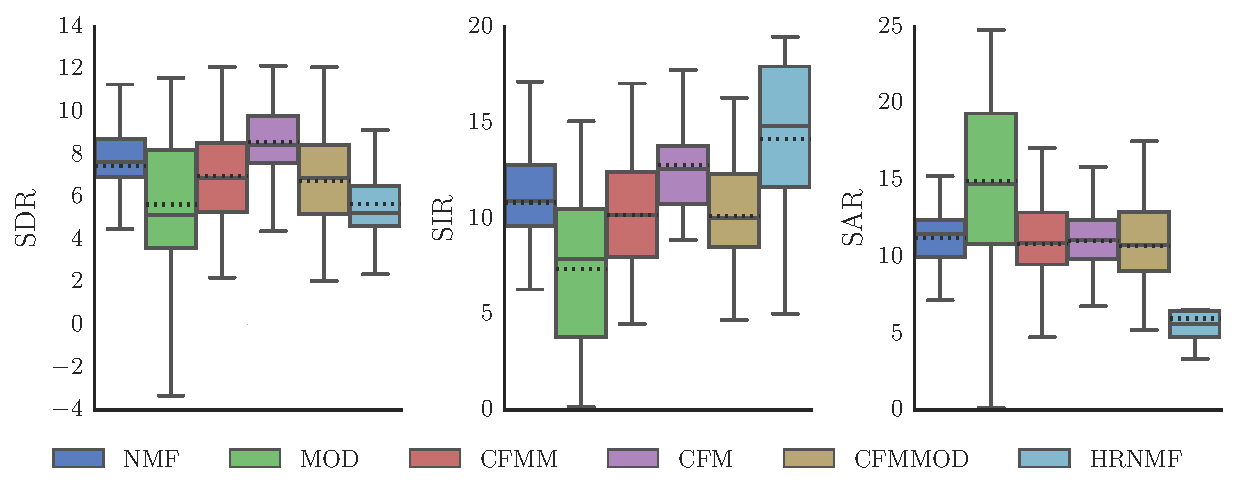
\includegraphics[width=0.8\textwidth]{Chapters/06_Separation_Unknown/figures/cfm_boxplot.pdf}
\caption{Boxplots of BSS-Eval results of the unison dataset. Solid/dotted lines represent medians/means. \textsuperscript{\textregistered}2016 IEEE.}
\label{fig:boxplot_overall}
\end{figure}

\begin{figure}[ht!]
\centering
        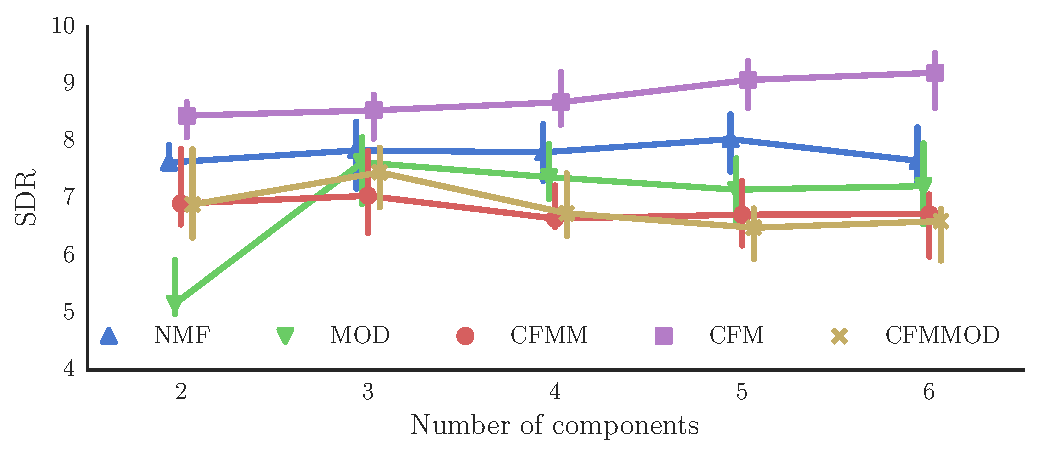
\includegraphics[width=0.8\textwidth]{Chapters/06_Separation_Unknown/figures/iterations.pdf}
\caption{Boxplots of SDR values of the unison dataset over the number of components $k$. For $k>2$ oracle clustering was applied. \textsuperscript{\textregistered}2016 IEEE.}
\label{fig:iterations}
\end{figure}

\section[Common Fate Transform for Music Separation]{Common Fate Transform\\for Music Separation}%
\label{sec:cft_for_lead_accompaniment_separation}

In the previous section, we showed that the Common Fate Model is suitable to separate highly overlapped signals based on their spatial-temporal modulation texture.
In this section, we want to show how this method can be extended for the application of vocal and accompaniment separation~\cite{rafii}.
This scenario is significantly more complex than the separation of instrument mixtures, hence the separation model needs to be flexible enough to handle many of the critical edge cases which make music separation challenging.
With the recent success of machine learning models~\cite{HintonSpeech}, it became likely that an unsupervised model such as NTF or CFM may not be flexible enough to enforce the significant amount of domain knowledge that is present in this scenario to improve performance.
Rafii et. al describe the current machine learning situation in \cite{rafii}:

\begin{quote}
  % TODO: make this look nicer
  ``Taking advantage of the recent availability of sufficiently large databases of isolated vocals along with their accompaniment, several researchers investigated the use of machine learning methods to directly estimate a mapping between the mixture and the sources~\cite{huang14, uhlich15}.
  However, most systems today still use classical time-frequency representations.

  The common structure of deep learning methods for lead and accompaniment separation usually corresponds to the one depicted in Figure~\ref{fig:methods_dnn}.
  Most methods mainly differ in the architecture picked for the network, its input, and output representation as well as in the way the network is trained.

  \begin{figure}
    \centering
    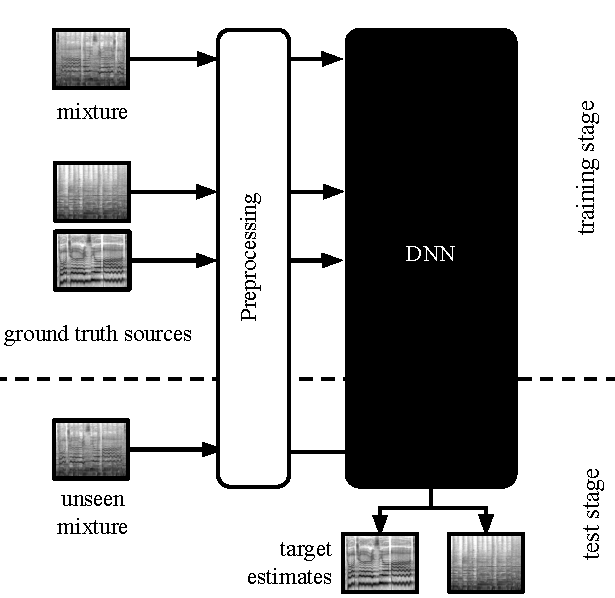
\includegraphics[width=0.6\textwidth]{Chapters/06_Separation_Unknown/figures/methods_dnn.pdf}
    \caption{General architecture for methods exploiting deep learning. The network inputs the mixture and outputs either the sources magnitude \acs{STFT} or a TF mask. Methods usually differ in their network architecture and the way use the training data for learning (a different version of this Figure was published in~\cite{rafii}). \textsuperscript{\textregistered}2018 IEEE.}
    \label{fig:methods_dnn}
  \end{figure}

  For the understanding of this section, it is sufficient to mention that DNNs consist of a cascade of several, possibly non-linear transformations of the input, which are learned during a training stage.
  They were shown to effectively learn representations and mappings, provided, enough data is available for estimating their parameters \cite{deng14, lecun15, goodfellow16}.
  Different architectures for neural networks may be combined/cascaded together, and many architectures were proposed in the past, such as \ac{FNN}, (\ac{CNN}), or \ac{RNN} and variants thereof such as the \ac{LSTM} and the gated-recurrent units (GRU).
  Training of such functions is achieved by stochastic gradient descent \cite{robbins51} and associated algorithms, such as backpropagation~\cite{rumelhart862} or backpropagation through time~\cite{rumelhart86} (BTT) for the case of \acs{RNN}s.
  \par
  Huang et al. were the first to propose \acs{RNN}s~\cite{hermans13,pascanu14} for singing voice separation in \cite{huang14,huang15}. They adapted their framework from \cite{huang142} to model all sources simultaneously through masking. Input and target functions were the mixture magnitude and a joint representation of the individual sources. The objective was to estimate jointly either singing voice and accompaniment music, or speech and background noise from the corresponding mixtures.
  \par
  Modeling the temporal structures of both the lead and the accompaniment is a considerable challenge. As an alternative to the \acs{RNN} approach proposed by Huang et al. in \cite{huang14}, Uhlich et al. proposed the usage of simpler \acs{FNN}s \cite{uhlich15} whose input consists of \textit{supervectors} stacked of few consecutive frames from the mixture.''
\end{quote}

We decided to reimplement Uhlich's model~\cite{uhlich15} to evaluate the separation quality.
The aim of this work was not to exactly reproduce the results, but instead, to evaluate one main research questions: does a DNN-based model benefit from the common fate representation being able to better capture the modulation texture?
For the implementation of the model, we used the Keras~\cite{chollet15} deep learning framework to systematically assess different combinations of input-and-output representation of the system.
\par
The network, as proposed in~\cite{uhlich15} consists of a three-layer fully connected network, where each of the hidden layers has the same number of hidden nodes as the targeted output representation.
This method can be described as a variant of a stacked denoising autoencoder~\cite{pvincent08}, where the noisy input is mapped to a clean output of the same dimensionality.
The architecture is depicted in Figure~\ref{fig:cft_dnn}. 

\begin{figure}[ht!]
\centering
        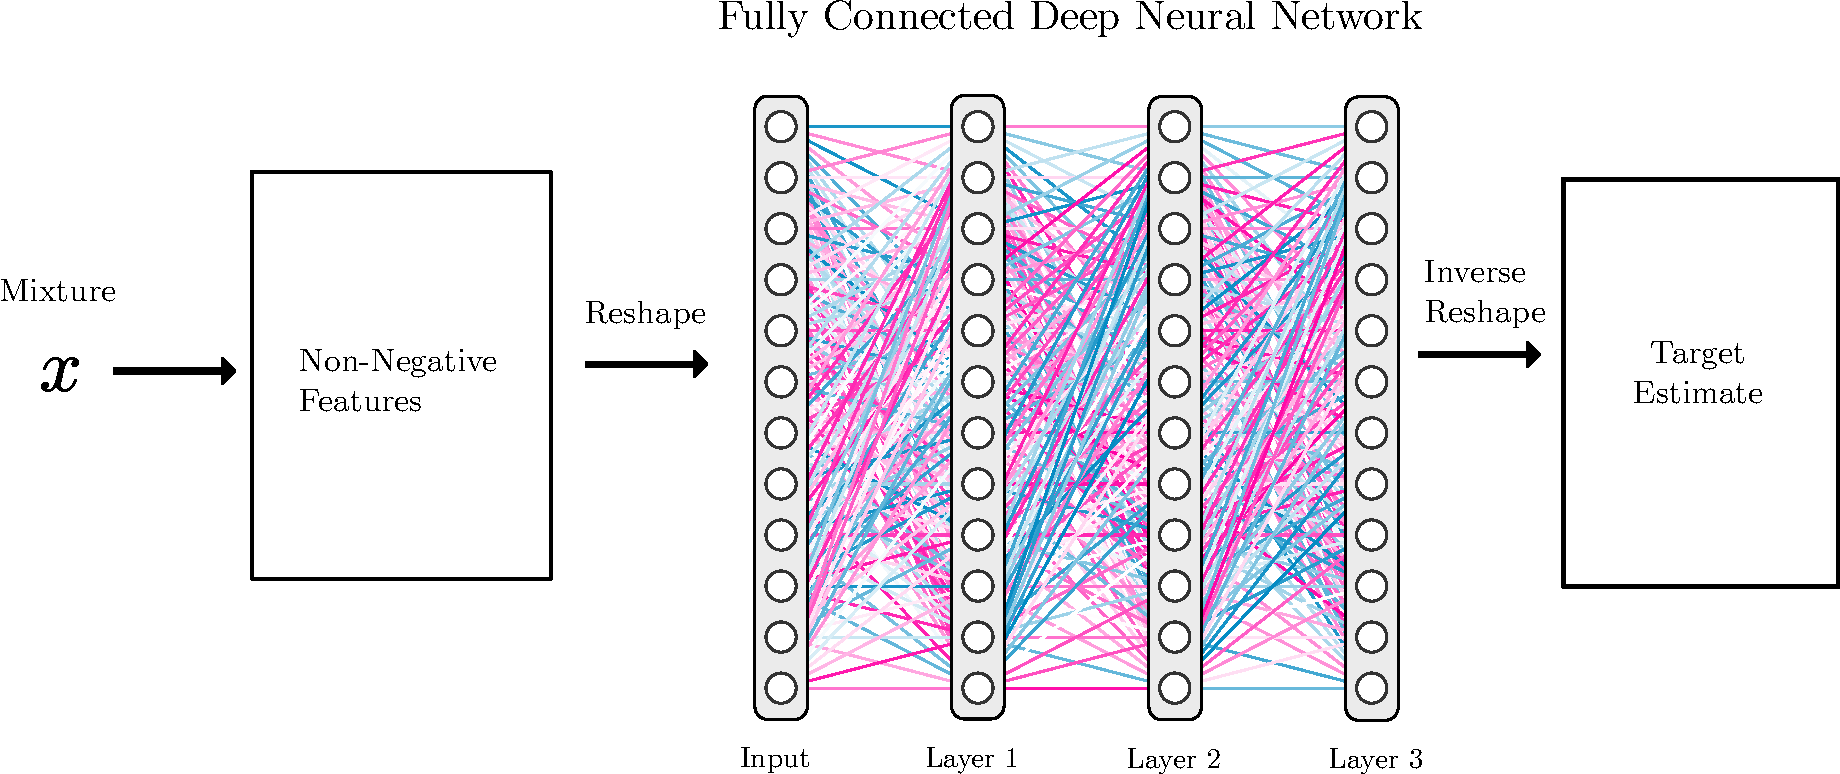
\includegraphics[width=\textwidth]{Chapters/06_Separation_Unknown/figures/uhlich_dnn.pdf}
\caption{Simplified block diagram of fully connected denoising autoencoder network as proposed by~\cite{uhlich15} for time-frequency based separation.}
\label{fig:cft_dnn}
\end{figure}

\subsection{Inputs and Outputs}

The purpose of the model is to create a non-linear mapping function from the magnitude of the input mixture \(\mX\) to the magnitude of the target source \(\mY_j\).
The optimal parameters (weights) \(\theta_j\) of such a mapping function \(\mY_j = f_{\theta_j}(\mX)\) are learned via supervised training.
\acs{FNN} networks, such as the one used here, can only deal with temporal structure by reshaping the time-frequency input to a super vector to be processed by the \acs{FNN}. 
However, this drawback is compensated by a large number of parameters in an \acs{FNN} layer.

Since the \acs{STFT}, GFT and CFT are lapped transforms, different scenarios for the input and output representation of the \acs{FNN} can be envisioned:

\begin{description}[style=unboxed,leftmargin=0cm]
\item[STFT-STFT]: for the \emph{input}, we computed the \acs{STFT} (\(N=1024, Hop=512\)) of each the audio track and selected excerpts of size, \(\mathbf{X} \in \mathcal{R}^{2C + 1}_{+} \), where \(C\) is the number of preceding and succeeding frames around the central frame \(\mathbf{X}_{i+C}\). For the \emph{output}, only a single central frame \(\mathbf{Y}_{i+C}\) is selected.
We used \(C=2\), reflecting the setting in~\cite{uhlich15}. This results in an input sample size of \(\mathbf{X} \in \mathcal{R}_{+}^{5 \times 513}\) and  \(\mathbf{Y} \in \mathcal{R}_{+}^{1 \times 513}\).

\item[GFT-GFT/GFT-STFT]: instead of taking excerpts from the \acs{STFT}, like in \emph{STFT-STFT}, we computed overlapping patches, as described in Section~\ref{sub:CFT}. Each patch is of size \((5, 8)\), which means that the same number of time frames are used compared to \emph{STFT-STFT} but additional redundancy has been added because of the overlap between neighboring patches.
For the \emph{output}, we chose the GFT of \(Y\).
This results in an input sample size of \(\mathbf{X} \in \mathcal{R}_{+}^{128 \times 5 \times 8}\) and  \(\mathbf{Y} \in \mathcal{R}_{+}^{128 \times 5 \times 8}\).
Furthermore, to reduce the number of parameters, we also evaluated a setting where just the \emph{output} is the central frame of the STFT.

\item[CFT-CFT/CFT-STFT]: in the first step, a processing as in \emph{GFT-GFT} was applied and then the 2D-DFT transform was applied (see Section~\ref{sub:CFT}).
This results in identical shapes as in the \emph{GFT-GFT} but with added benefits of this representation that can model neighboring phase dependencies.
\end{description}

We used the DSD100 dataset~\cite{ono15} for training and test. 
For each sample fed into the network, we randomly selected mixtures (without replacement) from the DSD100 dataset.

\subsection{Training}
We then sample from the DSD100 tracks and form single samples as input for the \acs{FNN}.
Therefore, we first compute the input representation of an audio track from the DSD100 set and then randomly sampling without replacement from these tracks.
The actual training has been done using mini-batches of size 32.
Each architecture is trained using the ADAM optimizer~\cite{kingma14} (learning rate: \(1 \cdot 10^{-3}\), \(\beta_1=0.9\), \(\beta_2=0.999\), \(\epsilon=1 \cdot 10^{-8}\))
The model was trained for a fixed number of 30 epochs and, in contrast to~\cite{uhlich15}, greedy layerwise pre-training was not applied.

\subsection{Results}

\begin{figure}[t]
\centering
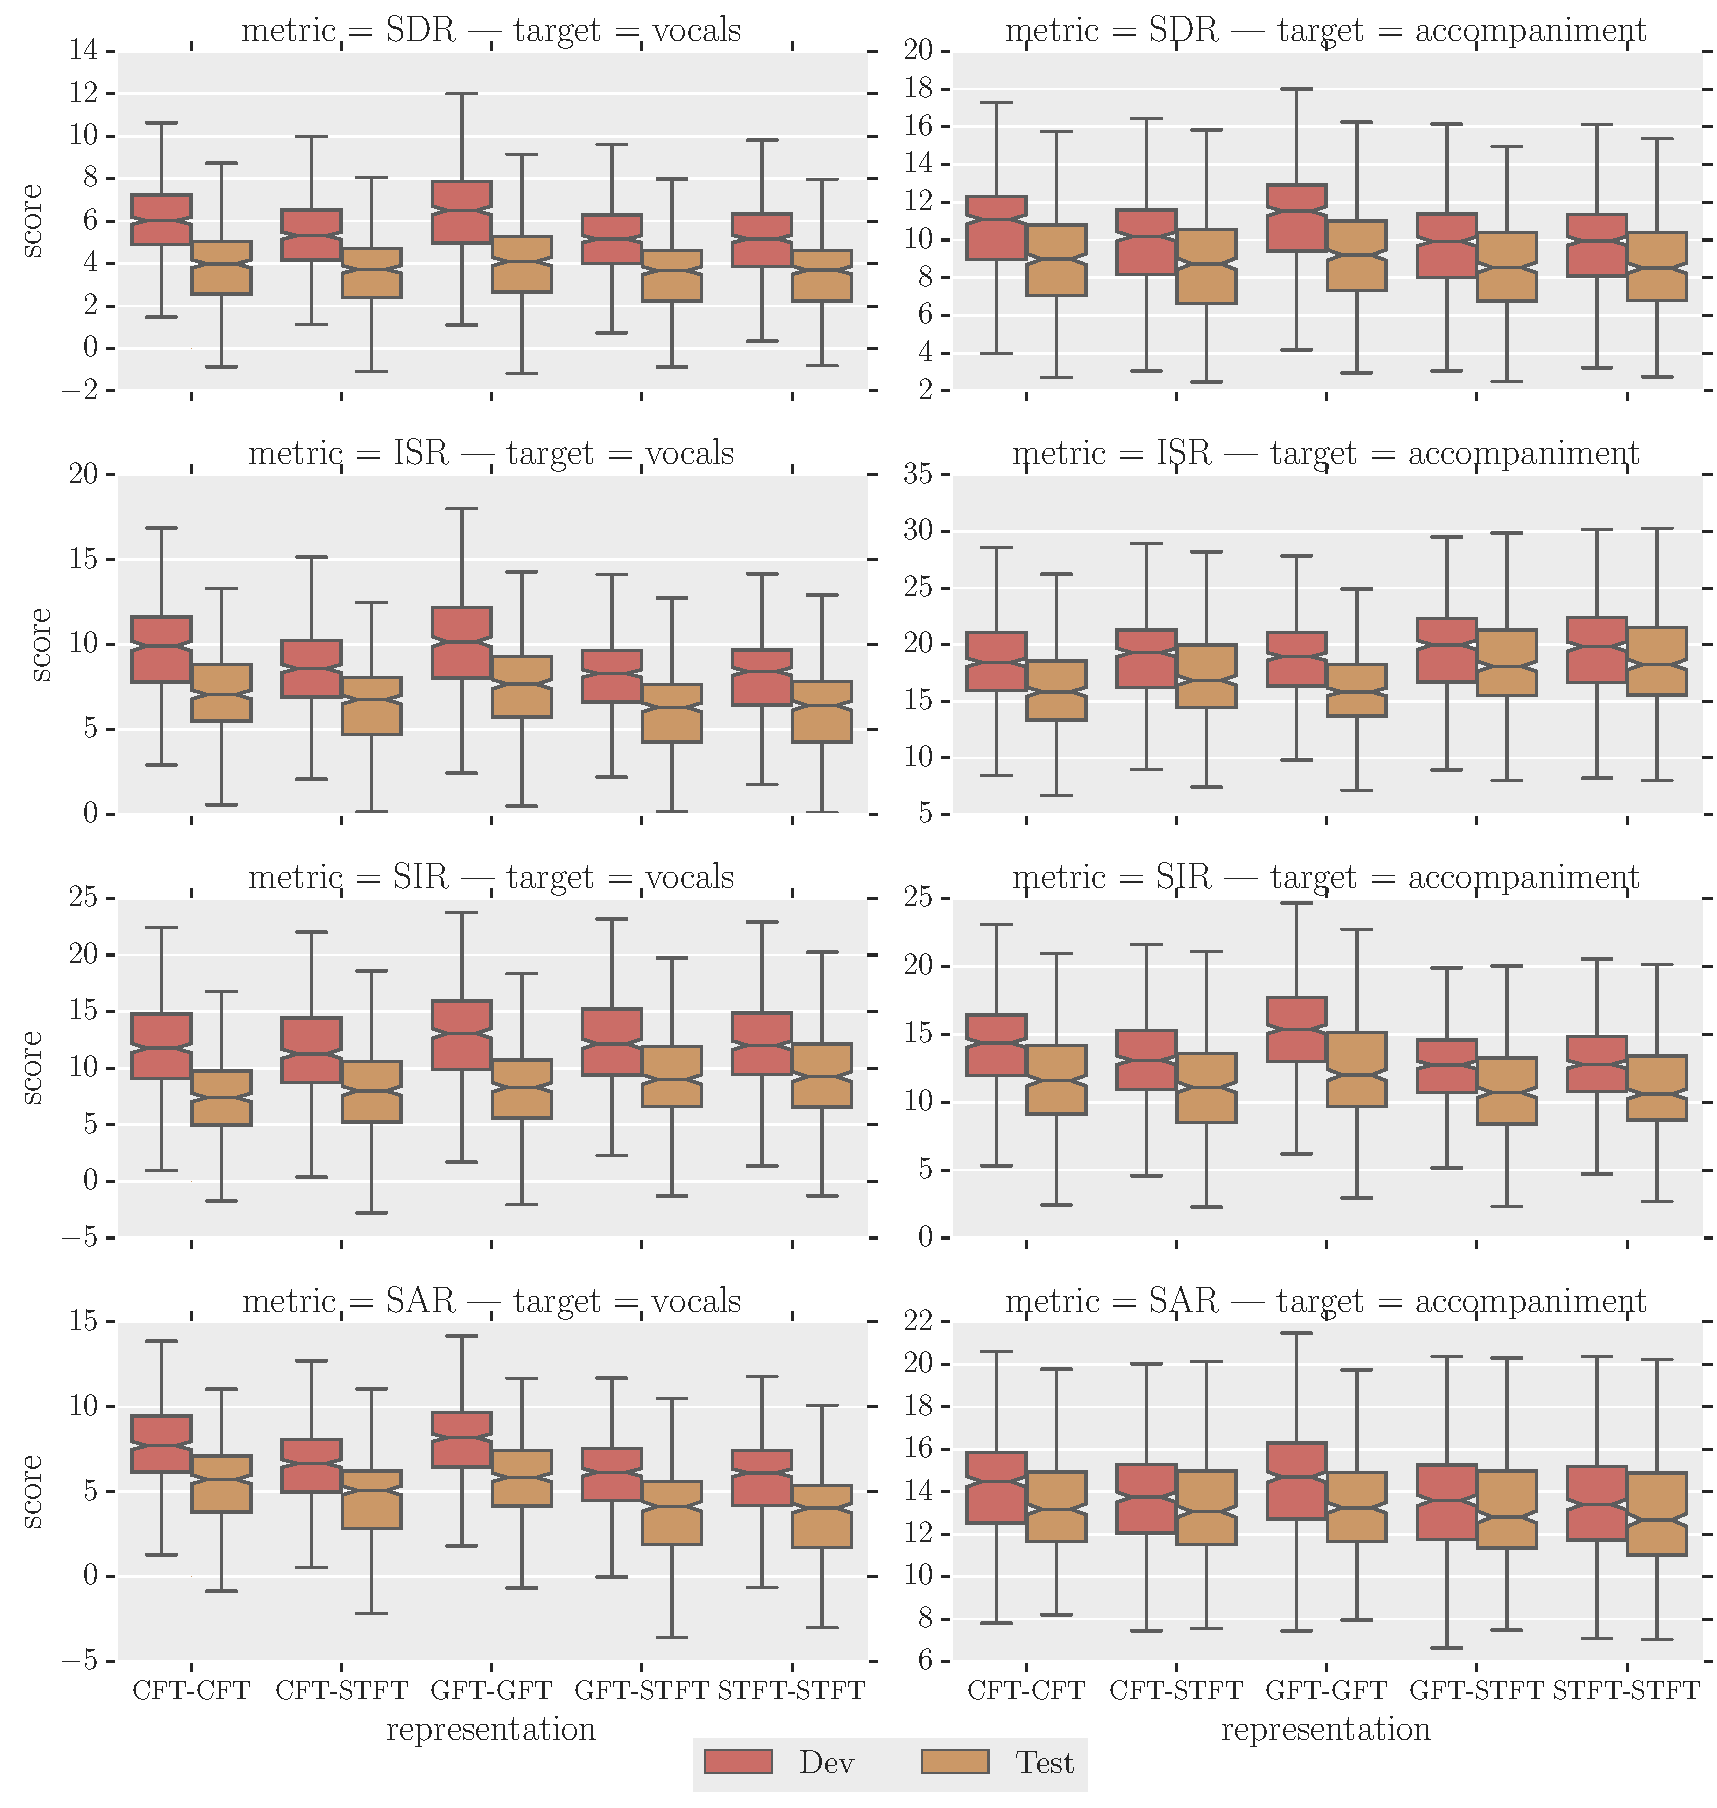
\includegraphics[width=1.1\textwidth]{Chapters/06_Separation_Unknown/figures/boxplot.pdf}
\caption{BSSEval separation results of the DSD100 dataset results for vocals and accompaniment sources. Several combinations of `input-output` were tested, as indicated by the x-axis.}
\label{fig:deep_cft_boxplots}
\end{figure}

For evaluation, the BSSEval metrics of all representations for the DSD100 test set were computed.
The results are depicted in Figure~\ref{fig:deep_cft_boxplots}.
They indicate that the common fate representation is indeed improving the baseline \emph{STFT-STFT} results.
Overall, we can report a mean difference of 0.4~dB for CFT-CFT and 0.5dB for GFT-GFT, compared to the \emph{STFT-STFT} representation.
However, it is worth mentioning that both, the GFT and the CFT representation lead to a significant increase in redundancy in the representation, thus increasing the number of trainable parameters per network layer (26 million for CFT vs 0.26 million for \acs{STFT}). Since we could not observe a large increase in difference of training (Dev) vs. test (Test) performance, we assume that the increasing number of parameters does not lead to large overfitting.

\subsection{Submission to SiSEC 2016}
\label{ssec:performance}

The results have been submitted to the 2016 \ac{SiSEC}~\cite{sisec16}.
This enables to relate the work compared to $22$ other source separation methods, all evaluated on the same test data, as part of the task for separating professionally-produced music recordings at \acs{SiSEC} 2016.
Table~\ref{tab:sisec_systems} lists the participating systems.
\begin{table*}[htbp]
  \centering
  \scriptsize
    \begin{tabular}{lll@{}}
        \hline
        \textbf{Acronym} & \textbf{Ref.} & \textbf{Summary}\\
        \hline
        STO1 & Proposed & \acs{FNN} on GFT representation \\
        STO2 & Proposed & \acs{FNN} on CFT representation \\
        HUA & \cite{huang12} & RPCA standard version \\
        RAF1 & \cite{rafii13} & REPET standard version \\
        RAF2 & \cite{liutkus12} & REPET with time-varying period \\
        RAF3 & \cite{rafii12} & REPET with similarity matrix \\
        KAM1-2 & \cite{liutkus15} & KAM with different configurations \\
        CHA & \cite{chan15} & RPCA with vocal activation information \\
        JEO1-2 & \cite{jeong17} &  $l_1$-RPCA with vocal activation information \\
        DUR & \cite{durrieu11} & Source-filter NMF \\
        OZE & \cite{salaun14} & Structured NMF with learned dictionaries \\
        KON & \cite{huang15} & \acs{RNN} \\
        GRA2-3 & \cite{grais16} & \acs{DNN} ensemble \\
        UHL1 & \cite{uhlich15} & \acs{FNN} with context \\
        NUG1-4 & \cite{nugraha16} & \acs{FNN} with multichannel information \\
        UHL2-3 & \cite{uhlich17} & \acs{LSTM} with multichannel information \\
        IBM & & ideal binary mask \\
  \end{tabular}
     \caption{Methods evaluated in \acs{SiSEC} 2016.}
    \label{tab:sisec_systems}

\end{table*}

%announcing the results and the webpage
The objective scores for my proposed methods were obtained using BSSEval and are given in Figure~\ref{fig:eval}.

\begin{figure*}[htbp]
    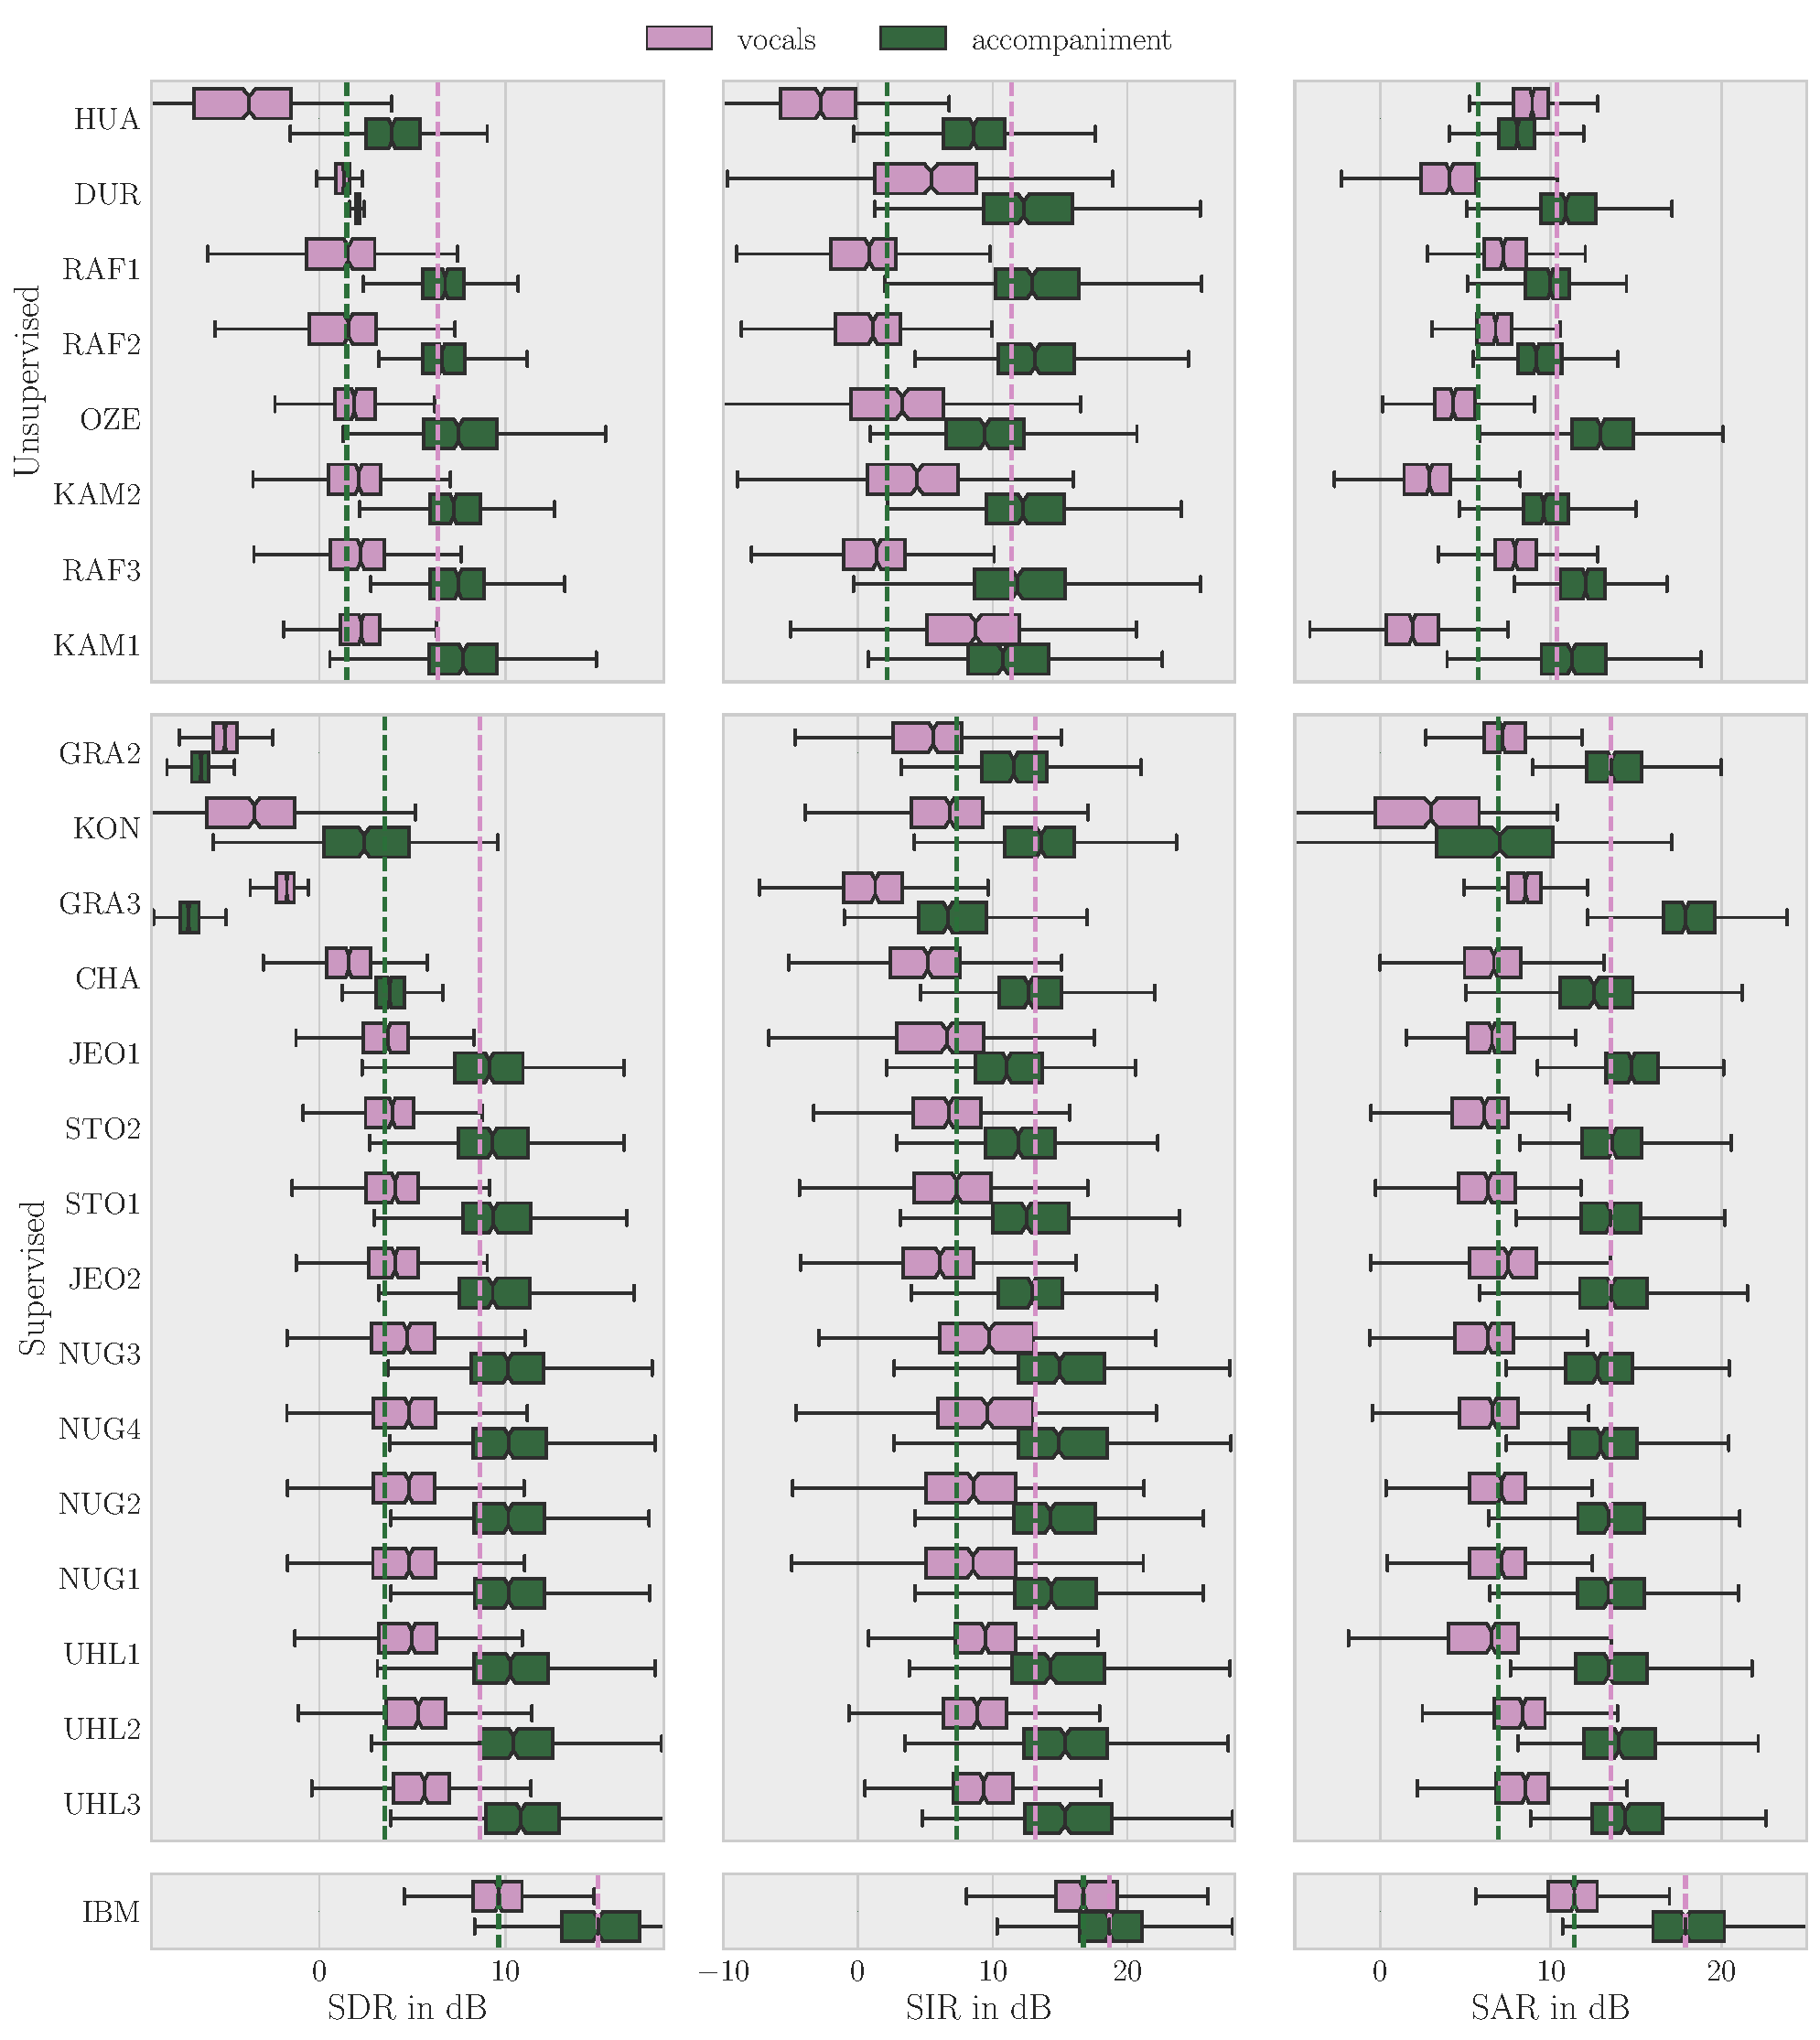
\includegraphics[width=1.1\textwidth]{Chapters/06_Separation_Unknown/figures/evaluation.pdf}
    \caption{BSSEval scores for the vocals and accompaniment estimates for \acs{SiSEC} 2016 on the DSD100 test dataset. Scores are sorted according the vocal median SDR and grouped by supervised and unsupervised methods. The proposed systems are \emph{STO1}, based on GFT-GFT and \emph{STO2}, based on CFT-CFT. Dashed lines indicate respective group medians.}
    \label{fig:eval}
\end{figure*}

% Maybe want to rewrite as it has been stolen from zafar
An obvious observation in Figure~\ref{fig:eval} is the difference in performance between data-driven methods and ``classical'' unsupervised methods. 
Further, it shows that exploiting learning data does help separation compared to only relying on \textit{a priori} assumptions such as the harmonicity or redundancy. 
Additionally, dynamic models such as LSTM from UHL2-3 appear more adapted to music than \acs{FNN}. 
These good performances in audio source separation go in line with the success of \acs{DNN}s in fields as varied as computer vision, speech recognition, and natural language processing \cite{lecun15}.
\par
Relating our results of STO1 and STO2 to the other methods, we observe that the performance was only slightly below the two state-of-the-art performances of UHL and NUG.
Furthermore, the difference between test and validation dataset indicates, that our CFT \acs{DNN} model even has better generalization as the one in NUG. 
While our STO model shares the same network architecture with UHL1, we were unable to reproduce the results, as we are approximately 1~dB below UHL1.
One reason is in the difference in initialization of the model as well as the fact that NUG and UHL models exploit multichannel information. 

\subsection{Evaluation Website}
\label{ssec:evaluation Website}

For more details and the ability for playback of the estimates, we refer to the dedicated interactive website that we built as part of my organizational help for \acs{SiSEC}\footnote{\url{http://www.sisec17.audiolabs-erlangen.de}}.
In fact, for the first time, interested researchers are now able to listen to over 10000 stimuli from all participating systems.
This was made possible through modern JavaScript technologies like the Web Audio API to interactively assess source separation results in the browser.
For each track, separation results are provided as well as the objective BSSeval scores, all of the data is reproducible and was made available in~\cite{oss_sisecwebsite}.
Figure~\ref{fig:sisec_website} depicts a screenshot of the website.
The objective scores are depicted as an interactive matrix where users are able to sort the results for each track and each system interactively by the source of interest.
Clicking on one rectangle in the heatmap opens the interactive player that allows to simultaneously playback the separated sources including changing the volume of each source.

\begin{figure}[!h]
\centering
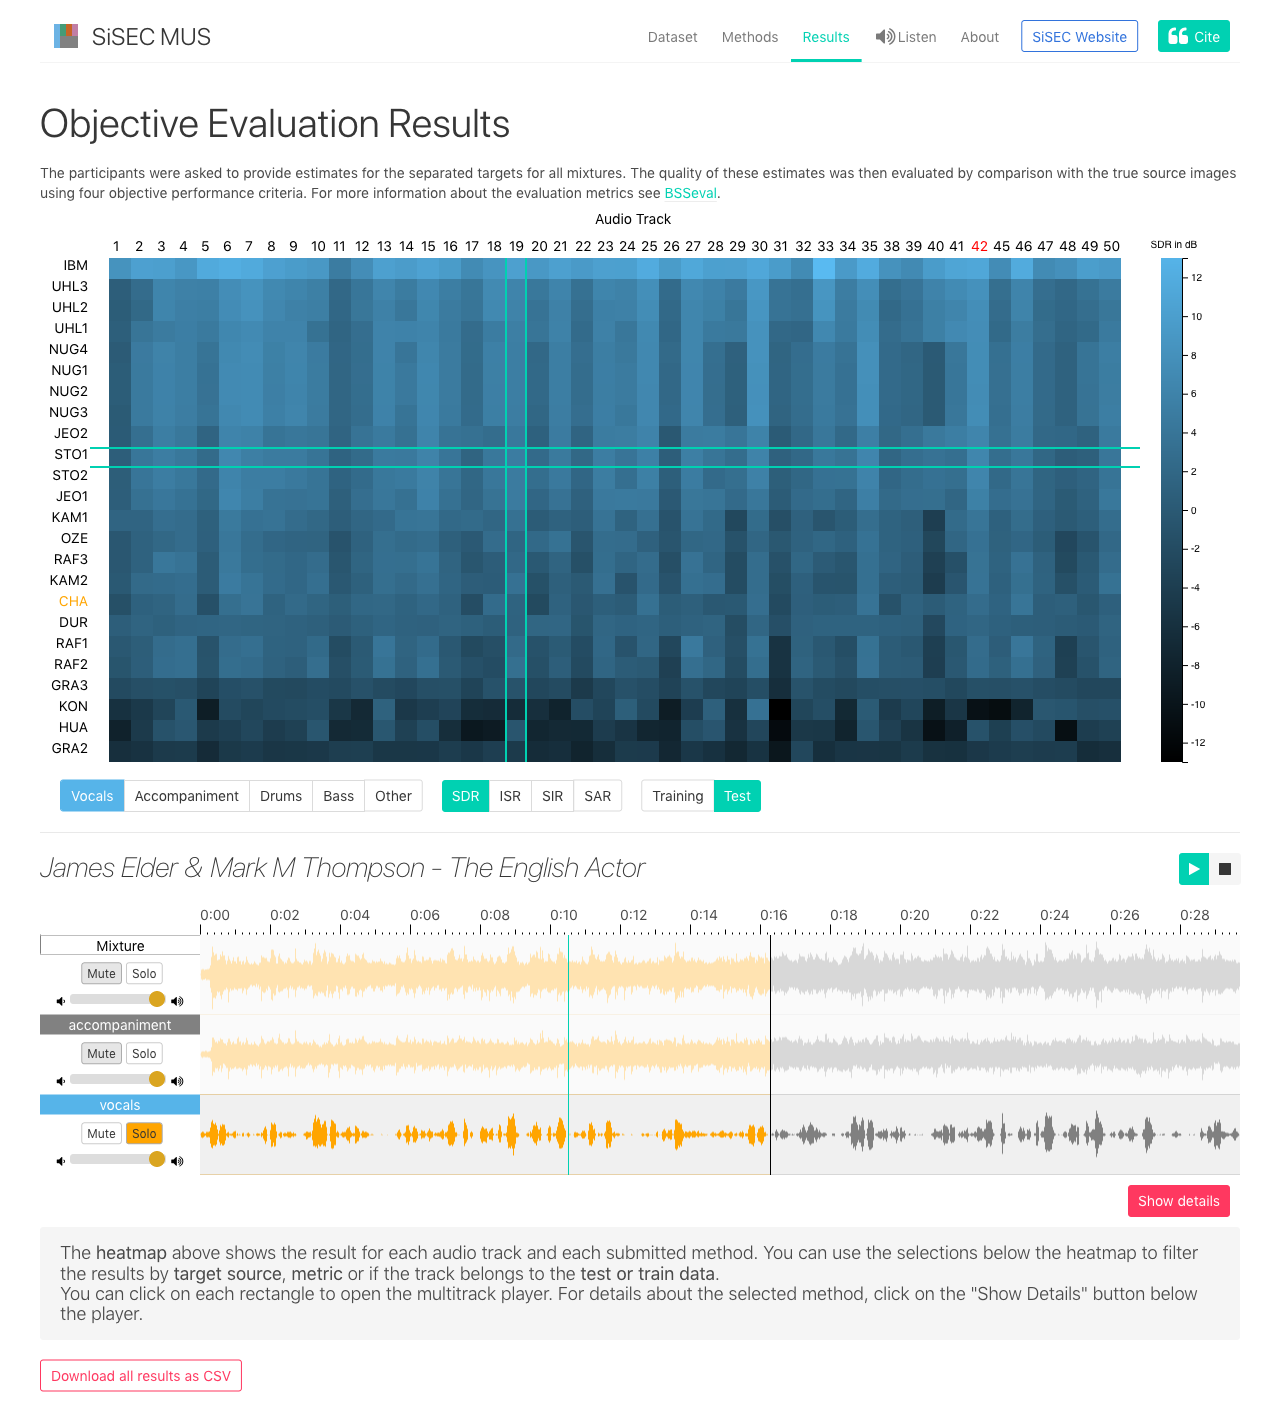
\includegraphics[width=0.9\textwidth]{Chapters/06_Separation_Unknown/figures/sisec_website.png}
\caption{Screenshot of the \acs{SiSEC} 2016 Website~\url{http://sisec17.audiolabs-erlangen.de}}
\label{fig:sisec_website}

\end{figure}

\section{Summary and Discussion}

In this chapter, we presented methods that exploit modulations for source separation without knowing them a priori. 
In the first part of this chapter, we presented a study where we demonstrated the use of the modulation spectrogram tensors for separating unison instrument mixtures, comparing the results with those presented in the previous chapter.
In a next step, we proposed a complex tensor representation, the Common Fate Transform (CFT), computed from rectangular patches of the complex \acs{STFT} using two-dimensional DFTs.
This novel representation exposes joint modulation characteristics of amplitude and frequency modulated signals while being fully invertible.
We demonstrated the usefulness of this representation using our Common Fate Model that factorizes patches from the CFT into two components, a modulation pattern and its activation. 
The model is inspired by the human's ability to group common modulations into single sources.
We presented results on unison musical instrument mixtures, indicating that it outperforms existing methods.
\par
In the second part of this chapter, we combined the CFT with an existing deep learning based separation model~\cite{uhlich15}.
We showed that the CFT improved separation quality compared to \acs{STFT} in a fully connected deep neural network.
Even though the CFT significantly increases the input size (due to its redundancy) and the number of trainable network parameters (due to its stacked auto-encoder architecture), generalization performance did not suffer.
\par
The results of the best performing model were submitted to \acs{SiSEC} 2016, where we scored among the top three participating research teams.
Finally, we presented interactive evaluation tools, developed for \acs{SiSEC}, allowing to interactively assess the performance of separation systems both objectively and subjectively.